\documentclass[aspectratio=169,9pt]{beamer}

% --- Theme: clean, robust (no external fonts, compiles with tectonic) ---
\usetheme{default}
\usecolortheme{seahorse}
\usefonttheme[onlymath]{serif}
\setbeamertemplate{navigation symbols}{}
\setbeamertemplate{itemize items}[circle]
\setbeamerfont{frametitle}{series=\bfseries}

\definecolor{accent}{RGB}{176,48,82}
\definecolor{ink}{RGB}{40,40,45}
\definecolor{soft}{RGB}{120,120,128}
\definecolor{good}{RGB}{30,110,70}
\definecolor{argA}{RGB}{40,95,165}
\definecolor{argB}{RGB}{190,140,20}
\definecolor{argC}{RGB}{125,60,150}
\setbeamercolor{frametitle}{fg=accent}
\setbeamercolor{structure}{fg=accent}
\setbeamercolor{normal text}{fg=ink}

\usepackage{amsmath,amssymb}
\usepackage{tikz}
\usetikzlibrary{arrows.meta,positioning,fit,backgrounds,calc,decorations.pathreplacing,patterns}
\usepackage{booktabs}
\usepackage{colortbl}
\usepackage{eqparbox}

\tikzset{
  box/.style={draw=accent!70, rounded corners, thick, fill=accent!6,
              inner sep=4pt, font=\scriptsize, align=center, minimum height=7mm},
  gate/.style={draw=soft, rounded corners, thin, fill=black!3,
              inner sep=3pt, font=\scriptsize, align=center},
  ghost/.style={draw=soft!60, rounded corners, thin, fill=black!2,
              inner sep=4pt, font=\scriptsize, align=center, minimum height=7mm, text=soft},
  flow/.style={-{Stealth[length=2mm]}, accent!80, thick},
}

\newcommand{\pending}[2][10.8cm]{%
  \begin{center}
  \begin{tikzpicture}
    \node[draw=soft, dashed, thick, rounded corners, fill=black!2,
          text width=#1, align=center, inner sep=7pt, font=\scriptsize]
      {\textbf{\textcolor{soft}{PENDING --- }}\textcolor{soft}{#2}};
  \end{tikzpicture}
  \end{center}}

\newcommand{\act}[2]{%
  \begin{frame}[plain]
    \centering \vfill
    {\Large\bfseries\color{accent} #1}\\[4pt]
    {\small #2}
    \vfill
  \end{frame}}

\newcommand{\subact}[2]{%
  \begin{frame}[plain]
    \centering \vfill
    {\large\bfseries\color{accent} #1}\\[4pt]
    {\small\color{soft} #2}
    \vfill
  \end{frame}}

\newcommand{\redlast}[1]{\multicolumn{1}{>{\columncolor{accent!14}[\tabcolsep][0pt]}c@{}}{#1}}
\newcommand{\seedtag}{g}
\newcommand{\seedpm}[2]{\eqmakebox[\seedtag M][r]{#1}\,{\tiny\color{soft}$\pm$\eqmakebox[\seedtag S][l]{#2}}}
\newcommand{\tintlast}[2]{\multicolumn{1}{>{\columncolor{#1}[\tabcolsep][0pt]}c@{}}{#2}}
\newcommand{\hleq}[1]{{\setlength{\fboxsep}{1.5pt}\colorbox{accent!12}{$\displaystyle #1$}}}
\newcommand{\hlval}[2]{{\setlength{\fboxsep}{1.2pt}\colorbox{#1}{\textcolor{white}{#2}}}}
\newcommand{\tintfirst}[2]{\multicolumn{1}{@{}>{\columncolor{#1}[0pt][0pt]}l}{#2\hspace{5pt}}}
\newcommand{\denomhl}[1]{{\setlength{\fboxsep}{1.5pt}\colorbox{accent!14}{$#1$}}}


\begin{document}

% motivation (short deck only)
\begin{frame}{Motivation: more area from the same flight time}
  \begin{columns}[c]
    \begin{column}{0.46\textwidth}
      \centering
      \resizebox{\linewidth}{!}{%
      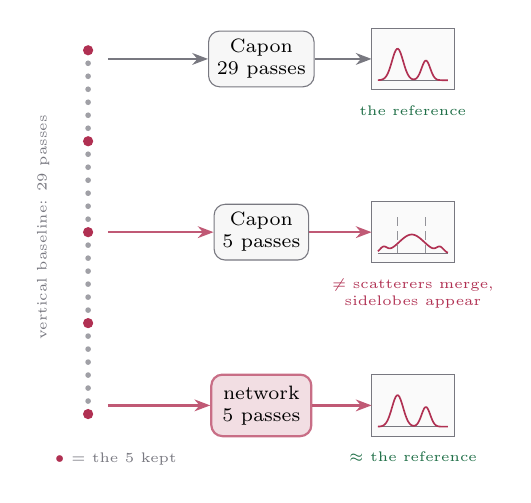
\begin{tikzpicture}[font=\scriptsize]
        \node[font=\tiny,text=soft,rotate=90,anchor=south] at (-0.12,0.06) {vertical baseline: 29 passes};
        \foreach \i in {1,...,29} \fill[soft!70] (0.25,{-2.31+0.165*(\i-1)}) circle (0.036);
        \foreach \i in {1,8,15,22,29} \fill[accent] (0.25,{-2.31+0.165*(\i-1)}) circle (0.065);
        \node[font=\tiny,text=soft,anchor=north west] at (-0.30,-2.68) {\textcolor{accent}{$\bullet$} $=$ the 5 kept};
        \node[gate,minimum height=7mm] (cfull) at (2.45,2.20) {Capon\\29 passes};
        \node[gate,minimum height=7mm] (cred)  at (2.45,0.00) {Capon\\5 passes};
        \node[box,fill=accent!16,minimum height=7mm] (net) at (2.45,-2.20) {network\\5 passes};
        \draw[flow,soft] (0.50,2.20) -- (cfull.west);
        \draw[flow] (0.50,0.00) -- (cred.west);
        \draw[flow] (0.50,-2.20) -- (net.west);
        \draw[soft,thin,fill=black!2] (3.85,1.81) rectangle ++(1.05,0.78);
        \draw[soft,thin] (3.93,1.93) -- (4.82,1.93);
        \draw[accent,semithick] plot[domain=3.93:4.82,samples=60] (\x,{1.93+0.40*exp(-(\x-4.18)^2/0.010)+0.25*exp(-(\x-4.54)^2/0.006)});
        \draw[flow,soft] (cfull.east) -- (3.85,2.20);
        \node[font=\tiny,text=good,anchor=north] at (4.375,1.73) {the reference};
        \draw[soft,thin,fill=black!2] (3.85,-0.39) rectangle ++(1.05,0.78);
        \draw[soft,thin] (3.93,-0.27) -- (4.82,-0.27);
        \draw[soft!80,densely dashed,thin] (4.18,-0.27) -- (4.18,0.24);
        \draw[soft!80,densely dashed,thin] (4.54,-0.27) -- (4.54,0.24);
        \draw[accent,semithick] plot[domain=3.93:4.82,samples=70] (\x,{-0.27+0.24*exp(-(\x-4.36)^2/0.050)+0.07*exp(-(\x-4.00)^2/0.004)+0.07*exp(-(\x-4.72)^2/0.004)});
        \draw[flow] (cred.east) -- (3.85,0.00);
        \node[font=\tiny,text=accent,anchor=north,align=center] at (4.375,-0.47) {$\neq$ scatterers merge,\\sidelobes appear};
        \draw[soft,thin,fill=black!2] (3.85,-2.59) rectangle ++(1.05,0.78);
        \draw[soft,thin] (3.93,-2.47) -- (4.82,-2.47);
        \draw[accent,semithick] plot[domain=3.93:4.82,samples=60] (\x,{-2.47+0.40*exp(-(\x-4.18)^2/0.010)+0.25*exp(-(\x-4.54)^2/0.006)});
        \draw[flow] (net.east) -- (3.85,-2.20);
        \node[font=\tiny,text=good,anchor=north] at (4.375,-2.67) {$\approx$ the reference};
      \end{tikzpicture}}
    \end{column}
    \begin{column}{0.50\textwidth}
      \centering
      \resizebox{\linewidth}{!}{%
      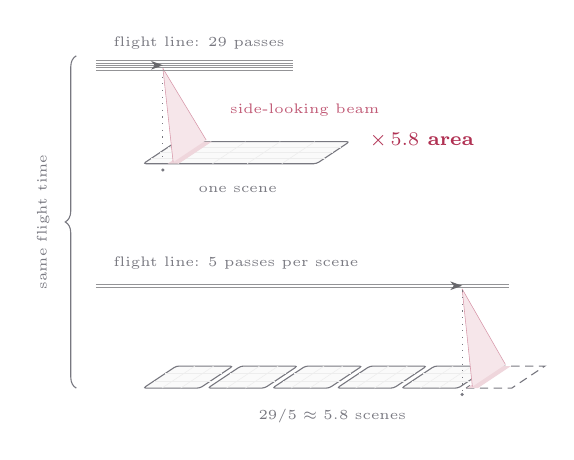
\begin{tikzpicture}[font=\scriptsize]
        \node[font=\tiny,text=soft,anchor=south west] at (0,1.33) {flight line: 29 passes};
        \draw[soft,thin,rounded corners=1pt,fill=black!2] (0.5,0) -- (2.7,0) -- (3.12,0.28) -- (0.92,0.28) -- cycle;
        \foreach \f in {0.25,0.5,0.75} \draw[black!7,very thin] ({0.5+\f*0.42},{\f*0.28}) -- ({2.7+\f*0.42},{\f*0.28});
        \foreach \g in {0.2,0.4,0.6,0.8} \draw[black!7,very thin] ({0.5+\g*2.2},0) -- ({0.5+\g*2.2+0.42},0.28);
        \fill[accent!20] (0.81,0) -- (0.95,0) -- (1.37,0.28) -- (1.23,0.28) -- cycle;
        \fill[accent!12] (0.75,1.21) -- (0.88,0.02) -- (1.30,0.30) -- cycle;
        \draw[accent!50,very thin] (0.75,1.21) -- (0.88,0.02);
        \draw[accent!50,very thin] (0.75,1.21) -- (1.30,0.30);
        \draw[soft,dotted,thin] (0.75,1.19) -- (0.75,-0.08);
        \fill[soft] (0.75,-0.08) circle (0.022);
        \foreach \o in {-0.06,-0.03,0,0.03,0.06} \draw[ink!50,very thin] (-0.1,{1.25+\o}) -- (2.4,{1.25+\o});
        \fill[ink!70] (0.75,1.25) -- ++(-0.15,0.055) -- ++(0.045,-0.055) -- ++(-0.045,-0.055) -- cycle;
        \node[font=\tiny,text=accent!80,anchor=west] at (1.48,0.68) {side-looking beam};
        \node[font=\tiny,text=soft,anchor=north] at (1.7,-0.16) {one scene};
        \node[font=\scriptsize\bfseries,text=accent,anchor=west] at (3.25,0.30) {$\times\,5.8$ area};
        \node[font=\tiny,text=soft,anchor=south west] at (0,-1.47) {flight line: 5 passes per scene};
        \foreach \x in {0.5,1.32,2.14,2.96,3.78} {
          \draw[soft,thin,rounded corners=1pt,fill=black!2] (\x,-2.85) -- ++(0.72,0) -- ++(0.42,0.28) -- ++(-0.72,0) -- cycle;
          \foreach \f in {0.33,0.66} \draw[black!7,very thin] ({\x+\f*0.42},{-2.85+\f*0.28}) -- ({\x+0.72+\f*0.42},{-2.85+\f*0.28});
          \foreach \g in {0.33,0.66} \draw[black!7,very thin] ({\x+\g*0.72},-2.85) -- ({\x+\g*0.72+0.42},-2.57);
        }
        \draw[soft,thin,densely dashed] (4.60,-2.85) -- ++(0.58,0) -- ++(0.42,0.28) -- ++(-0.58,0) -- cycle;
        \fill[accent!20] (4.61,-2.85) -- (4.75,-2.85) -- (5.17,-2.57) -- (5.03,-2.57) -- cycle;
        \fill[accent!12] (4.55,-1.59) -- (4.68,-2.83) -- (5.10,-2.55) -- cycle;
        \draw[accent!50,very thin] (4.55,-1.59) -- (4.68,-2.83);
        \draw[accent!50,very thin] (4.55,-1.59) -- (5.10,-2.55);
        \draw[soft,dotted,thin] (4.55,-1.61) -- (4.55,-2.93);
        \fill[soft] (4.55,-2.93) circle (0.022);
        \foreach \o in {-0.025,0.025} \draw[ink!50,very thin] (-0.1,{-1.55+\o}) -- (5.15,{-1.55+\o});
        \fill[ink!70] (4.55,-1.55) -- ++(-0.15,0.055) -- ++(0.045,-0.055) -- ++(-0.045,-0.055) -- cycle;
        \node[font=\tiny,text=soft,anchor=north] at (2.9,-2.99) {$29/5 \approx 5.8$ scenes};
        \draw[decorate,decoration={brace,amplitude=4pt},soft] (-0.35,-2.85) -- (-0.35,1.37);
        \node[font=\tiny,text=soft,rotate=90,anchor=south] at (-0.57,-0.74) {same flight time};
      \end{tikzpicture}}
    \end{column}
  \end{columns}
\end{frame}

% full deck p.3 --- sections/01_overview.tex
\begin{frame}{Methodology}
  \centering
  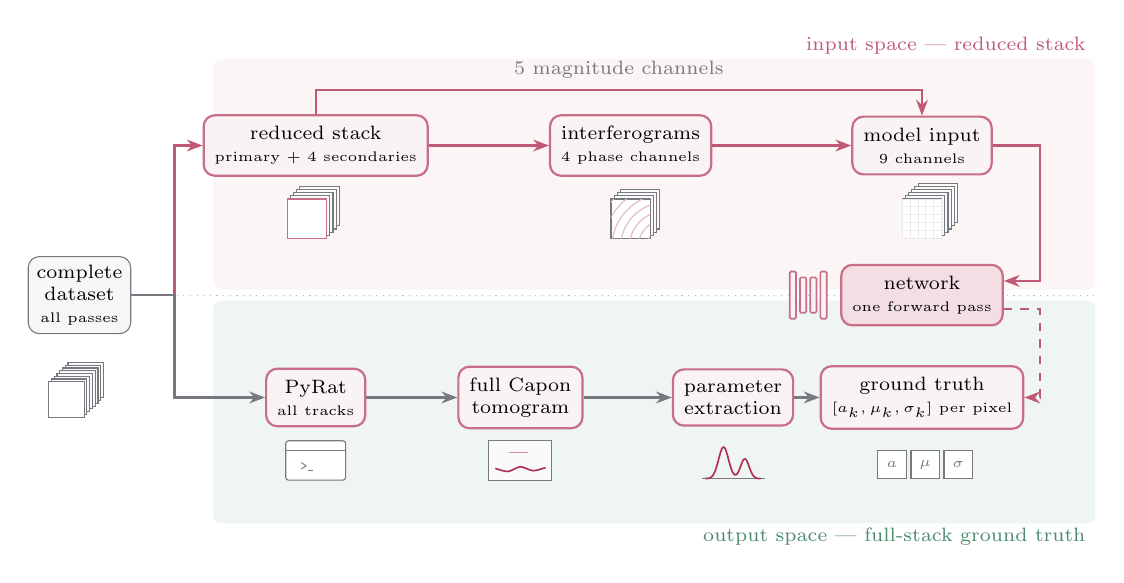
\begin{tikzpicture}
    \begin{scope}[on background layer]
      \fill[accent!5,rounded corners=3pt] (1.7,0.07) rectangle (12.9,3.0);
      \fill[good!7,rounded corners=3pt] (1.7,-0.07) rectangle (12.9,-2.9);
      \draw[soft!50,dotted] (-0.2,0) -- (12.9,0);
    \end{scope}
    \node[font=\scriptsize,text=accent!80,anchor=east] at (12.9,3.17) {input space --- reduced stack};
    \node[font=\scriptsize,text=good!80,anchor=east] at (12.9,-3.07) {output space --- full-stack ground truth};
    \node[gate] (ds) at (0,0) {complete\\dataset\\{\tiny all passes}};
    \foreach \i in {7,6,5,4,3,2,1} \draw[soft,thin,fill=black!2] (-0.39+0.035*\i,-1.55+0.035*\i) rectangle ++(0.45,0.45);
    \draw[soft,thin,fill=white] (-0.39,-1.55) rectangle ++(0.45,0.45);
    \node[box] (top1) at (3.0,1.9) {reduced stack\\{\tiny primary + 4 secondaries}};
    \foreach \i in {4,3,2,1} \draw[soft,thin,fill=black!2] (2.64+0.04*\i,0.72+0.04*\i) rectangle ++(0.5,0.5);
    \draw[accent!70,thin,fill=white] (2.64,0.72) rectangle ++(0.5,0.5);
    \node[box] (top2) at (7.0,1.9) {interferograms\\{\tiny 4 phase channels}};
    \foreach \i in {3,2,1} \draw[soft,thin,fill=black!2] (6.75+0.04*\i,0.72+0.04*\i) rectangle ++(0.5,0.5);
    \draw[soft,thin,fill=white] (6.75,0.72) rectangle ++(0.5,0.5);
    \begin{scope} \clip (6.75,0.72) rectangle ++(0.5,0.5); \foreach \r in {0.25,0.36,...,0.95} \draw[accent!35,thin] (7.45,0.6) circle (\r); \end{scope}
    \node[box] (top3) at (10.7,1.9) {model input\\{\tiny 9 channels}};
    \foreach \i in {5,4,3,2,1} \draw[soft,thin,fill=black!2] (10.45+0.04*\i,0.72+0.04*\i) rectangle ++(0.5,0.5);
    \draw[soft,thin,fill=white] (10.45,0.72) rectangle ++(0.5,0.5);
    \draw[black!8,step=0.1,shift={(10.45,0.72)}] (0,0) grid (0.5,0.5);
    \node[box, fill=accent!16] (net) at (10.7,0) {network\\{\tiny one forward pass}};
    \foreach \x/\h in {9.02/0.6,9.15/0.45,9.28/0.45,9.41/0.6} \draw[accent!70,semithick,fill=accent!6,rounded corners=0.5pt] (\x,-\h/2) rectangle ++(0.08,\h);
    \node[box] (bot1) at (3.0,-1.3) {PyRat\\{\tiny all tracks}};
    \draw[soft,thin,rounded corners=1pt,fill=white] (2.62,-2.35) rectangle ++(0.76,0.5);
    \draw[soft,thin] (2.62,-1.97) -- (3.38,-1.97);
    \node[font=\tiny,text=soft,anchor=west] at (2.68,-2.18) {\texttt{>\_}};
    \node[box] (bot2) at (5.6,-1.3) {full Capon\\tomogram};
    \draw[soft,thin,fill=black!2] (5.2,-2.35) rectangle ++(0.8,0.5);
    \draw[accent,semithick] plot[smooth] coordinates {(5.28,-2.20) (5.44,-2.24) (5.60,-2.18) (5.76,-2.23) (5.92,-2.19)};
    \draw[accent!55,semithick] (5.45,-2.00) -- (5.70,-2.00);
    \node[box] (bot3) at (8.3,-1.3) {parameter\\extraction};
    \draw[soft,thin] (7.9,-2.33) -- (8.7,-2.33);
    \draw[accent,semithick] plot[domain=7.95:8.65,samples=60] (\x,{-2.33+0.4*exp(-(\x-8.18)^2/0.008)+0.25*exp(-(\x-8.45)^2/0.006)});
    \node[box] (gt) at (10.7,-1.3) {ground truth\\{\tiny $[a_k,\mu_k,\sigma_k]$ per pixel}};
    \foreach \x/\lbl in {10.14/{$a$},10.56/{$\mu$},10.98/{$\sigma$}} { \draw[soft,thin,fill=white] (\x,-2.33) rectangle ++(0.36,0.36); \node[font=\tiny,text=soft] at (\x+0.18,-2.15) {\lbl}; }
    \draw[flow] (ds.east) -- ++(0.55,0) |- (top1.west);
    \draw[flow, soft] (ds.east) -- ++(0.55,0) |- (bot1.west);
    \draw[flow] (top1) -- (top2);
    \draw[flow] (top2) -- (top3);
    \draw[flow] (top1.north) -- (3.0,2.6) -- (10.7,2.6) -- (top3.north);
    \node[font=\scriptsize,text=soft,anchor=south] at (6.85,2.63) {5 magnitude channels};
    \draw[flow] (top3.east) -| (12.2,0.18) -- ([yshift=0.18cm]net.east);
    \draw[flow, soft] (bot1) -- (bot2);
    \draw[flow, soft] (bot2) -- (bot3);
    \draw[flow, soft] (bot3) -- (gt);
    \draw[flow, dashed] ([yshift=-0.18cm]net.east) -- (12.2,-0.18) |- (gt.east);
  \end{tikzpicture}
  \\[8pt]
  \small
  A network learns to reconstruct, from the \textbf{reduced} stack alone,\\
  the per-pixel profile parameters that the full-stack tomogram and classical fit produce.
\end{frame}

% full deck p.14 --- sections/03_dataset_labels.tex
\begin{frame}{Ground truth: fitted Gaussian parameters}
  \small
  \begin{columns}[T]
    \begin{column}{0.55\textwidth}
      \begin{minipage}[t][0.68\textheight]{\linewidth}
      \vfill
      Supervised target: the per-pixel array $[a_k,\mu_k,\sigma_k]_{k=1}^{K}$
      ($K{=}2$ today, $K{=}5$ in development), fit to the per-pixel max-normalised
      Capon spectrum $\tilde p = p/p_{\max}$ on the elevation grid $\xi_n$:
      \[
        \mathcal{L} \;=\; \frac{1}{N}\sum_{n=1}^{N}\big(\hat p(\xi_n)-\tilde p(\xi_n)\big)^{2},
        \qquad
        \hat p(\xi) = \sum_{k} a_k\, e^{-\frac{(\xi-\mu_k)^2}{2\sigma_k^2}}
      \]
      \vfill
      One shared loss; each parameter group takes its own projected Adam step:
      \[
        \begin{aligned}
          a_k      &\;\leftarrow\; \big[\, a_k - \eta\,\mathrm{Adam}(\partial_{a_k}\mathcal{L}) \,\big]_{+} \\[-1pt]
          \mu_k    &\;\leftarrow\; \operatorname{clip}_{[\mu^-\!,\;\mu^+]}\big( \mu_k - \eta\,\mathrm{Adam}(\partial_{\mu_k}\mathcal{L}) \big) \\[-1pt]
          \sigma_k &\;\leftarrow\; \operatorname{clip}_{[\sigma^-\!,\;\sigma^+]}\big( \sigma_k - \eta\,\mathrm{Adam}(\partial_{\sigma_k}\mathcal{L}) \big)
        \end{aligned}
      \]
      \vfill
      \end{minipage}
    \end{column}
    \begin{column}{0.43\textwidth}
      \centering
      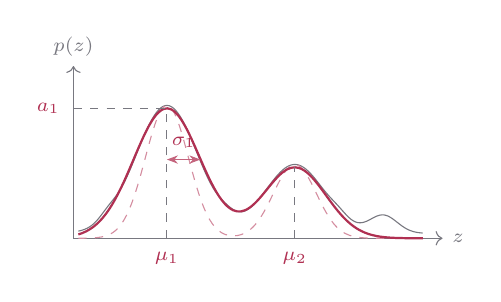
\begin{tikzpicture}[scale=1.25]
        \draw[->,soft] (0,0) -- (3.75,0) node[right,font=\scriptsize]{$z$};
        \draw[->,soft] (0,0) -- (0,1.75) node[above,font=\scriptsize]{$p(z)$};
        \draw[soft,thin,domain=0.05:3.55,samples=160,smooth]
          plot (\x,{1.30*exp(-(\x-0.95)^2/(2*0.10)) + 0.70*exp(-(\x-2.25)^2/(2*0.09))
                    + 0.18*exp(-(\x-3.15)^2/(2*0.02)) + 0.06*exp(-(\x-0.35)^2/(2*0.008))
                    + 0.04*exp(-(\x-1.55)^2/(2*0.008)) + 0.04*exp(-(\x-2.70)^2/(2*0.008)) + 0.05});
        \draw[accent!55,thin,dashed,domain=0.05:3.55,samples=90,smooth]
          plot (\x,{1.35*exp(-(\x-0.95)^2/(2*0.048)) + 0.75*exp(-(\x-2.25)^2/(2*0.048))});
        \draw[accent,thick,domain=0.05:3.55,samples=90,smooth]
          plot (\x,{1.32*exp(-(\x-0.95)^2/(2*0.115)) + 0.72*exp(-(\x-2.25)^2/(2*0.10))});
        \draw[soft,dashed,thin] (0.95,0) -- (0.95,1.32);
        \draw[soft,dashed,thin] (2.25,0) -- (2.25,0.72);
        \draw[soft,dashed,thin] (0,1.32) -- (0.95,1.32);
        \draw[{Stealth[length=1.4mm]}-{Stealth[length=1.4mm]},accent!75,thin]
          (0.95,0.80) -- (1.29,0.80);
        \node[font=\scriptsize,accent,anchor=north] at (0.95,-0.04) {$\mu_1$};
        \node[font=\scriptsize,accent,anchor=north] at (2.25,-0.04) {$\mu_2$};
        \node[font=\scriptsize,accent,anchor=east]  at (-0.04,1.32) {$a_1$};
        \node[font=\scriptsize,accent,anchor=south] at (1.12,0.82) {$\sigma_1$};
      \end{tikzpicture}
      \\[2pt]
      {\scriptsize Same pixel: \textcolor{soft}{Capon spectrum},
       \textcolor{accent!60}{peak initialisation (dashed)},
       \textcolor{accent}{converged fit}; the fitted $[a_k,\mu_k,\sigma_k]$ are the label.}
      \begin{itemize}
        \item {\footnotesize Fitted in normalised space; the winning amplitudes are
              denormalised back, $a_k \to p_{\max}\, a_k$ ($\mu_k$, $\sigma_k$ already
              live on the physical axis).}
        \item {\footnotesize All pixels batched in one optimisation --- not a per-pixel
              loop (next slide); most pixels activate one or two Gaussians (Act III).}
      \end{itemize}
    \end{column}
  \end{columns}
\end{frame}

% main-results agenda (short deck only)
\begin{frame}{Main results}
  \begin{itemize}\setlength{\itemsep}{12pt}
    \item \textbf{Hungarian matching}: assigning predicted scatterers to ground-truth scatterers (next frame).
    \item \textbf{Set-prediction head}: gated slots that decide existence and parameters per scatterer.
    \item \textbf{Receptive field}: how much spatial context the network actually uses.
    \item \textbf{Benchmarking}: 7 backbones $\times$ 5 objectives, five seeds each: the board.
    \item \textbf{Dual backbone}: two trunks, one head: existence and parameters each get their own encoder.
    \item \textbf{Pair loss function}: param-L1 paired with a curve term.
  \end{itemize}
\end{frame}

% full deck p.33 --- sections/06_set_prediction.tex
\begin{frame}{Hungarian matching}
  \small
  \begin{columns}[c]
    \begin{column}{0.5\textwidth}
      \begin{itemize}
        \item Each Gaussian is a \textbf{point in $(a,\mu,\sigma)$ space}: prediction and
              GT are two point sets; the matcher pairs them by distance and scores the
              \emph{set}, not the slot layout.
      \end{itemize}
      \vspace{6pt}
      \centering
      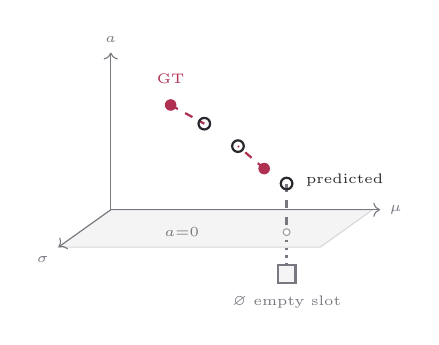
\begin{tikzpicture}[scale=0.95, every node/.style={font=\tiny}]
        \begin{scope}[on background layer]
          \fill[soft!8] (0,0) -- (3.5,0) -- (2.8,-0.5) -- (-0.7,-0.5) -- cycle;
          \draw[soft!30, thin] (0,0) -- (3.5,0) -- (2.8,-0.5) -- (-0.7,-0.5) -- cycle;
        \end{scope}
        \node[soft] at (0.95,-0.30) {$a{=}0$};
        \draw[->,soft] (0,0) -- (3.6,0) node[right]{$\mu$};
        \draw[->,soft] (0,0) -- (0,2.1) node[above]{$a$};
        \draw[->,soft] (0,0) -- (-0.7,-0.5) node[below left]{$\sigma$};
        \draw[accent, dashed, thick] (0.8,1.4) -- (1.25,1.15);
        \draw[accent, dashed, thick] (2.05,0.55) -- (1.7,0.85);
        \draw[soft, dashed, thick] (2.35,0.35) -- (2.35,-0.30);
        \draw[soft, dotted, thick] (2.35,-0.30) -- (2.35,-0.74);
        \fill[accent] (0.8,1.4) circle (2.2pt);
        \fill[accent] (2.05,0.55) circle (2.2pt);
        \draw[ink, thick] (1.25,1.15) circle (2.2pt);
        \draw[ink, thick] (1.7,0.85) circle (2.2pt);
        \draw[ink, thick] (2.35,0.35) circle (2.2pt);
        \draw[soft!70, fill=white] (2.35,-0.30) circle (1.3pt);
        \draw[soft, thick, fill=black!4] (2.23,-0.98) rectangle (2.47,-0.74);
        \node[accent, anchor=south] at (0.8,1.55) {GT};
        \node[ink, anchor=west] at (2.48,0.40) {predicted};
        \node[soft, anchor=north] at (2.35,-1.02) {$\varnothing$ empty slot};
      \end{tikzpicture}
      \\ {\scriptsize Filled = active GT, open = predicted, $\varnothing$ = empty GT slot
      (below $a{=}0$). Its match (grey) is zero-weighted, so $\hat\theta_3$ is free.}
    \end{column}
    \begin{column}{0.5\textwidth}
      \centering
      \[
        \mathcal{L} \;=\; \min_{\pi \in S_K}\ \sum_{k=1}^{K} w_k
          \left\| \hat\theta_{\pi(k)} - \theta_k \right\|^{2}
        \qquad \theta_k = (a_k,\mu_k,\sigma_k)
      \]
      {\scriptsize $w_k=\mathbf{1}[a_k>\tau]$ --- GT \emph{active mask}: $1$ if present, $0$ if empty.}\\[15pt]
      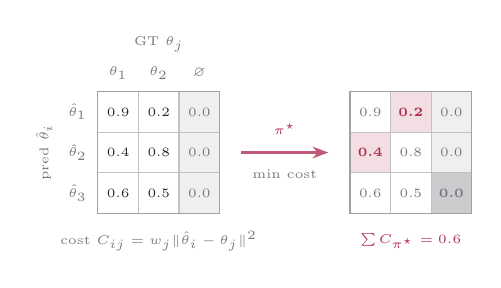
\begin{tikzpicture}[scale=0.92, transform shape, font=\tiny]
        % ===================== cost matrix =====================
        \node[text=soft] at (0.84,0.66) {GT $\theta_j$};
        \node[text=soft] at (0.28,0.26) {$\theta_1$};
        \node[text=soft] at (0.84,0.26) {$\theta_2$};
        \node[text=soft] at (1.40,0.26) {$\varnothing$};
        \node[text=soft, rotate=90] at (-0.74,-0.84) {pred $\hat\theta_i$};
        \node[text=soft] at (-0.28,-0.28) {$\hat\theta_1$};
        \node[text=soft] at (-0.28,-0.84) {$\hat\theta_2$};
        \node[text=soft] at (-0.28,-1.40) {$\hat\theta_3$};
        \fill[soft!12] (1.12,0) rectangle (1.68,-1.68);
        \draw[step=0.56, soft!45, thin] (0,-1.68) grid (1.68,0);
        \draw[soft!70] (0,-1.68) rectangle (1.68,0);
        \node[text=ink]  at (0.28,-0.28) {0.9};
        \node[text=ink]  at (0.84,-0.28) {0.2};
        \node[text=soft] at (1.40,-0.28) {0.0};
        \node[text=ink]  at (0.28,-0.84) {0.4};
        \node[text=ink]  at (0.84,-0.84) {0.8};
        \node[text=soft] at (1.40,-0.84) {0.0};
        \node[text=ink]  at (0.28,-1.40) {0.6};
        \node[text=ink]  at (0.84,-1.40) {0.5};
        \node[text=soft] at (1.40,-1.40) {0.0};
        \node[text=soft] at (0.84,-2.06) {cost $C_{ij}=w_j\lVert\hat\theta_i-\theta_j\rVert^{2}$};
        % ===================== arrow =====================
        \draw[flow] (1.98,-0.84) -- (3.18,-0.84);
        \node[text=accent] at (2.58,-0.52) {$\pi^\star$};
        \node[text=soft]   at (2.58,-1.14) {min cost};
        % ===================== selected matching =====================
        \begin{scope}[shift={(3.48,0)}]
          \fill[soft!12]   (1.12,0)      rectangle (1.68,-1.68);
          \fill[accent!16] (0.56,0)      rectangle (1.12,-0.56);
          \fill[accent!16] (0,-0.56)     rectangle (0.56,-1.12);
          \fill[soft!38]   (1.12,-1.12)  rectangle (1.68,-1.68);
          \draw[step=0.56, soft!45, thin] (0,-1.68) grid (1.68,0);
          \draw[soft!70] (0,-1.68) rectangle (1.68,0);
          \node[text=soft]   at (0.28,-0.28) {0.9};
          \node[text=accent] at (0.84,-0.28) {\textbf{0.2}};
          \node[text=soft]   at (1.40,-0.28) {0.0};
          \node[text=accent] at (0.28,-0.84) {\textbf{0.4}};
          \node[text=soft]   at (0.84,-0.84) {0.8};
          \node[text=soft]   at (1.40,-0.84) {0.0};
          \node[text=soft]   at (0.28,-1.40) {0.6};
          \node[text=soft]   at (0.84,-1.40) {0.5};
          \node[text=soft]   at (1.40,-1.40) {\textbf{0.0}};
          \node[text=accent] at (0.84,-2.06) {$\textstyle\sum C_{\pi^\star}=0.6$};
        \end{scope}
      \end{tikzpicture}\hspace*{2.5em}
      \\[4pt] {\scriptsize Column $\varnothing$ is a placeholder GT ($w_j{=}0$) --- all-zero,
      so the leftover prediction matches it for free:
      $\hat\theta_1\!\to\!\theta_2,\ \hat\theta_2\!\to\!\theta_1,\ \hat\theta_3\!\to\!\varnothing$.}
    \end{column}
  \end{columns}
\end{frame}

% full deck p.35 --- sections/06_set_prediction.tex
\begin{frame}{Inside the set-prediction head --- gate, blend, match}
  \small
  \begin{columns}[T]
    \begin{column}{0.56\textwidth}
      \centering
      \vspace{4pt}
      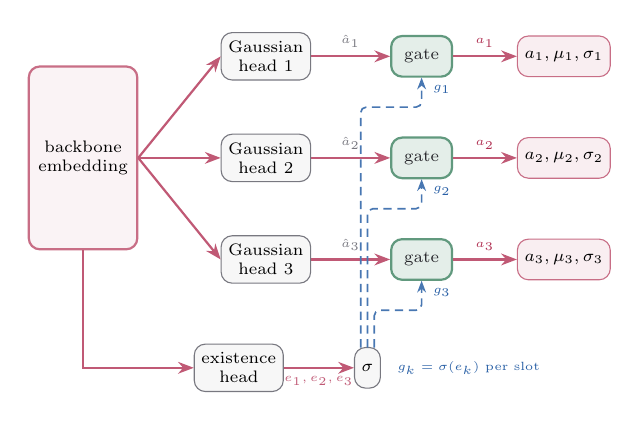
\begin{tikzpicture}[font=\scriptsize, scale=0.86, transform shape,
          exc/.style={-{Stealth[length=1.5mm]}, argA!85, semithick, densely dashed}]
        \node[box, minimum height=27mm, minimum width=16mm] (bb) at (0,0) {backbone\\embedding};
        \node[gate, minimum height=7mm] (h1) at (2.7,1.5)  {Gaussian\\head 1};
        \node[gate, minimum height=7mm] (h2) at (2.7,0)    {Gaussian\\head 2};
        \node[gate, minimum height=7mm] (h3) at (2.7,-1.5) {Gaussian\\head 3};
        \node[box, draw=good!70, fill=good!12, text=ink, minimum height=6mm, minimum width=9mm] (g1) at (5.0,1.5)  {gate};
        \node[box, draw=good!70, fill=good!12, text=ink, minimum height=6mm, minimum width=9mm] (g2) at (5.0,0)    {gate};
        \node[box, draw=good!70, fill=good!12, text=ink, minimum height=6mm, minimum width=9mm] (g3) at (5.0,-1.5) {gate};
        \node[gate, draw=accent!70, fill=accent!8, minimum height=6mm] (o1) at (7.1,1.5)  {$a_1,\mu_1,\sigma_1$};
        \node[gate, draw=accent!70, fill=accent!8, minimum height=6mm] (o2) at (7.1,0)    {$a_2,\mu_2,\sigma_2$};
        \node[gate, draw=accent!70, fill=accent!8, minimum height=6mm] (o3) at (7.1,-1.5) {$a_3,\mu_3,\sigma_3$};
        \node[gate, minimum height=7mm] (eh)  at (2.3,-3.1) {existence\\head};
        \node[gate, minimum height=6mm] (sig) at (4.2,-3.1) {$\sigma$};
        \draw[flow] (bb.east) -- (h1.west);
        \draw[flow] (bb.east) -- (h2.west);
        \draw[flow] (bb.east) -- (h3.west);
        \draw[flow] (bb.south) |- (eh.west);
        \draw[flow] (h1.east) -- node[midway, above, font=\tiny, text=soft]{$\hat a_1$} (g1.west);
        \draw[flow] (h2.east) -- node[midway, above, font=\tiny, text=soft]{$\hat a_2$} (g2.west);
        \draw[flow] (h3.east) -- node[midway, above, font=\tiny, text=soft]{$\hat a_3$} (g3.west);
        \draw[flow] (g1.east) -- node[midway, above, font=\tiny, text=accent]{$a_1$} (o1.west);
        \draw[flow] (g2.east) -- node[midway, above, font=\tiny, text=accent]{$a_2$} (o2.west);
        \draw[flow] (g3.east) -- node[midway, above, font=\tiny, text=accent]{$a_3$} (o3.west);
        \draw[flow] (eh.east) -- (sig.west) node[midway, below, font=\tiny]{$e_1,e_2,e_3$};
        \draw[exc, rounded corners=2pt] (4.10,-2.8) -- (4.10,0.75)  -| (g1.south);
        \draw[exc, rounded corners=2pt] (4.20,-2.8) -- (4.20,-0.75) -| (g2.south);
        \draw[exc, rounded corners=2pt] (4.30,-2.8) -- (4.30,-2.25) -| (g3.south);
        \node[font=\tiny, text=argA, anchor=north] at (5.3,1.2)  {$g_1$};
        \node[font=\tiny, text=argA, anchor=north] at (5.3,-0.3) {$g_2$};
        \node[font=\tiny, text=argA, anchor=north] at (5.3,-1.8) {$g_3$};
        \node[font=\tiny, text=argA, anchor=west] at ($(sig.east)+(0.12,0)$) {$g_k=\sigma(e_k)$ per slot};
      \end{tikzpicture}
      \\[8pt]
      {\footnotesize each gate:\; $a_k = g_k\,\hat a_k + (1-g_k)\,a_{\mathrm{off},k}$}\\[1pt]
      {\scriptsize\color{soft} $\mu_k,\sigma_k$ pass through $\cdot$ $a_{\mathrm{off}}$ learned per slot}
    \end{column}
    \begin{column}{0.44\textwidth}
      \footnotesize
      \textbf{The gate is a sigmoid} on the existence logit $e_k$:
      \begin{itemize}\setlength{\itemsep}{5pt}
        \item Open slots ($g_k\!\to\!1$): $a_k \approx \hat a_k$ --- the raw regression survives.
        \item Closed slot ($g_k\!\to\!0$): $a_k \to a_{\mathrm{off},k}\approx 0$ \emph{whatever}
              $\hat a_k$ is, collapsing onto the empty-set target at near-zero loss.
        \item $e_k$ is internal --- the head still emits $3K$ channels $(a_k,\mu_k,\sigma_k)$;
              $a_{\mathrm{off}}$ is a learned per-slot scalar (init $0$).
      \end{itemize}
      \vspace{8pt}
      \centering
      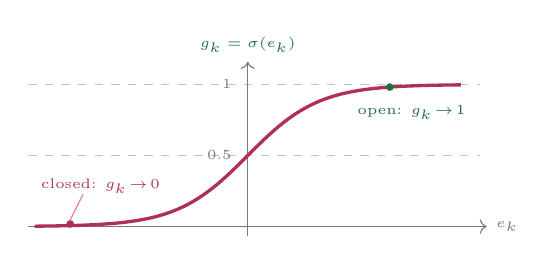
\begin{tikzpicture}[scale=0.82, font=\scriptsize]
        \draw[soft!45, dashed] (-3.4,2.2) -- (3.6,2.2);
        \draw[soft!45, dashed] (-3.4,1.1) -- (3.6,1.1);
        \node[soft, font=\tiny, anchor=east] at (-0.1,2.2) {1};
        \node[soft, font=\tiny, anchor=east] at (-0.1,1.1) {0.5};
        \draw[->, soft] (-3.4,0) -- (3.7,0) node[right, font=\tiny]{$e_k$};
        \draw[->, soft] (0,-0.15) -- (0,2.55) node[above, font=\tiny, text=good]{$g_k=\sigma(e_k)$};
        \draw[accent, very thick, samples=90, domain=-6:6] plot ({\x*0.55},{2.2/(1+exp(-\x))});
        \fill[good] (2.2,2.16) circle (1.7pt);
        \node[good, font=\tiny, anchor=north west] at (1.55,2.02) {open: $g_k\!\to\!1$};
        \fill[accent] (-2.75,0.04) circle (1.7pt);
        \node[accent, font=\tiny, anchor=west] at (-3.35,0.62) {closed: $g_k\!\to\!0$};
        \draw[accent!60, thin] (-2.75,0.1) -- (-2.55,0.5);
      \end{tikzpicture}
    \end{column}
  \end{columns}
\end{frame}

% full deck p.61 --- sections/08_context_information.tex
\begin{frame}{Reading the reach --- the network estimates statistics}
  \begin{columns}[c]
    \begin{column}{0.05\textwidth}
    \end{column}
    \begin{column}{0.42\textwidth}
      \centering
      {\scriptsize two labels at offset $\Delta$ split into shared and
       private looks:\par}
      \vspace{4pt}
      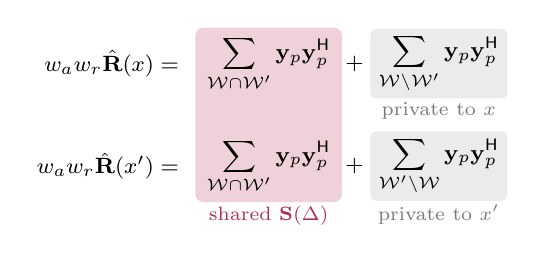
\begin{tikzpicture}[font=\footnotesize, baseline,
          box/.style={rounded corners=2pt, inner xsep=3pt, inner ysep=2pt},
          lbl/.style={font=\scriptsize, inner sep=1pt, anchor=north}]
        \node[anchor=east] (ex) at (0,0)    {$w_{a}w_{r}\hat{\mathbf R}(x) =$};
        \node[anchor=east] (ey) at (0,-1.3) {$w_{a}w_{r}\hat{\mathbf R}(x') =$};
        \node[box, anchor=west] (sx) at (0.12,0)    {$\displaystyle\sum_{\mathcal W\cap\mathcal W'}\mathbf y_p\mathbf y_p^{\mathsf H}$};
        \node[box, anchor=west] (sy) at (0.12,-1.3) {$\displaystyle\sum_{\mathcal W\cap\mathcal W'}\mathbf y_p\mathbf y_p^{\mathsf H}$};
        \node[anchor=west, inner xsep=2pt] (px) at (sx.east) {$+$};
        \node[anchor=west, inner xsep=2pt] (py) at (sy.east) {$+$};
        \node[box, fill=black!8, anchor=west] (dx) at (px.east) {$\displaystyle\sum_{\mathcal W\setminus\mathcal W'}\mathbf y_p\mathbf y_p^{\mathsf H}$};
        \node[box, fill=black!8, anchor=west] (dy) at (py.east) {$\displaystyle\sum_{\mathcal W'\setminus\mathcal W}\mathbf y_p\mathbf y_p^{\mathsf H}$};
        \begin{scope}[on background layer]
          \node[fit=(sx)(sy), fill=accent!22, rounded corners=3pt, inner sep=1pt] (sh) {};
        \end{scope}
        \node[lbl, text=accent, anchor=north] at (sh.south) {shared $\mathbf S(\Delta)$};
        \node[lbl, text=soft] at (dx.south) {private to $x$};
        \node[lbl, text=soft] at (dy.south) {private to $x'$};
      \end{tikzpicture}\\[12pt]
      {\scriptsize the shared fraction at every offset $\tau$ is the
       correlation law:\par}
      \vspace{2pt}
      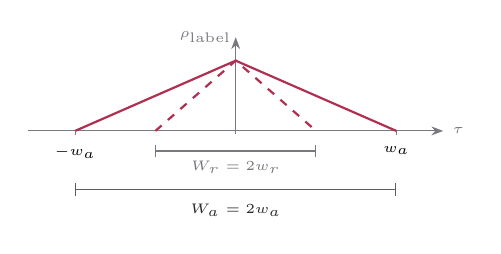
\begin{tikzpicture}[scale=0.85]
        \draw[-{Stealth[length=1.5mm]}, soft] (-3.1,0) -- (3.1,0) node[right,font=\tiny]{$\tau$};
        \draw[-{Stealth[length=1.5mm]}, soft] (0,-0.05) -- (0,1.40)
          node[anchor=east, font=\tiny, inner sep=1.5pt]{$\rho_{\text{label}}$};
        \draw[accent, thick]         (-2.4,0) -- (0,1.05) -- (2.4,0);
        \draw[accent, thick, dashed] (-1.2,0) -- (0,1.05) -- (1.2,0);
        \draw[soft, thin] (-2.4,0) -- (-2.4,-0.06);
        \draw[soft, thin] (2.4,0) -- (2.4,-0.06);
        \node[font=\tiny, anchor=north] at (-2.4,-0.08) {$-w_{a}$};
        \node[font=\tiny, anchor=north] at (2.4,-0.08) {$w_{a}$};
        \draw[|-|, ink!75] (-2.4,-0.88) -- (2.4,-0.88);
        \node[font=\tiny, text=ink, anchor=north] at (0,-0.95) {$W_{a} = 2w_{a}$};
        \draw[|-|, soft] (-1.2,-0.30) -- (1.2,-0.30);
        \node[font=\tiny, text=soft, anchor=north] at (0,-0.30) {$W_{r} = 2w_{r}$};
      \end{tikzpicture}\\[2pt]
      {\scriptsize the label correlates over $\pm w_{a}$ in azimuth and
       $\pm w_{r}$ in range --- the centred patch spanning both triangles is
       $W_{a}{\times}W_{r}$.\par}
    \end{column}
    \begin{column}{0.51\textwidth}
      \centering
      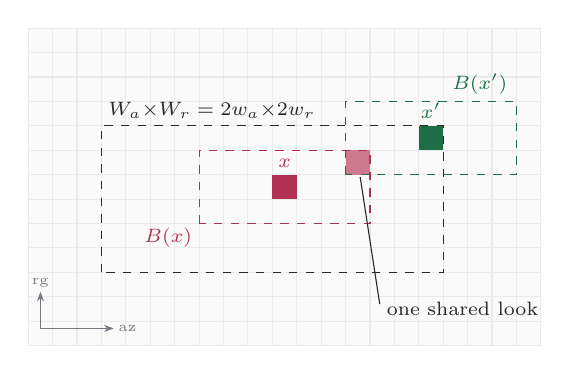
\begin{tikzpicture}[scale=1.55]
        \draw[soft, thin, fill=black!2] (0,0) rectangle (4.2,2.6);
        \draw[black!8, step=0.2] (0,0) grid (4.2,2.6);
        \fill[accent!65] (2.60,1.40) rectangle ++(0.2,0.2);
        \fill[accent] (2.00,1.20) rectangle ++(0.2,0.2);
        \fill[good] (3.20,1.60) rectangle ++(0.2,0.2);
        \draw[ink, dashed, thin] (0.60,0.60) rectangle ++(2.8,1.2);
        \node[font=\scriptsize, text=ink, anchor=south west, inner sep=1.5pt] at (0.62,1.82) {$W_{a}{\times}W_{r} = 2w_{a}{\times}2w_{r}$};
        \draw[accent, dashed, thin] (1.40,1.00) rectangle ++(1.4,0.6);
        \node[font=\scriptsize, text=accent, anchor=north east, inner sep=1.5pt] at (1.38,1.00) {$B(x)$};
        \node[font=\scriptsize, text=accent, anchor=south, inner sep=1.5pt] at (2.10,1.42) {$x$};
        \draw[good, dashed, thin] (2.60,1.40) rectangle ++(1.4,0.6);
        \node[font=\scriptsize, text=good, anchor=south, inner sep=1.5pt] at (3.70,2.02) {$B(x')$};
        \node[font=\scriptsize, text=good, anchor=south, inner sep=1.5pt] at (3.30,1.82) {$x'$};
        \node[font=\scriptsize, text=ink, anchor=west, inner sep=1.5pt] at (2.90,0.30) {one shared look};
        \draw[ink, thin] (2.88,0.34) -- (2.72,1.38);
        \draw[-{Stealth[length=1.2mm]}, soft] (0.10,0.14) -- (0.70,0.14)
          node[right, font=\tiny, inner sep=1.5pt] {az};
        \draw[-{Stealth[length=1.2mm]}, soft] (0.10,0.14) -- (0.10,0.44)
          node[above, font=\tiny, inner sep=1.5pt] {rg};
      \end{tikzpicture}\\[4pt]
      {\scriptsize $x'$ sits at the far corner of the patch: $B(x')$ keeps a
       single shared look with $B(x)$ --- one step further and the windows are
       disjoint ($|\Delta_{a}| = w_{a}$ \emph{or} $|\Delta_{r}| = w_{r}$).}
    \end{column}
  \end{columns}
\end{frame}

% full deck p.78 --- sections/10_benchmark_board.tex
\newcommand{\sspm}[2]{\eqmakebox[bbSM][r]{#1}\,{\tiny\color{soft}$\pm$\eqmakebox[bbSS][l]{#2}}}
\begin{frame}{The board at five seeds --- the L1 family owns the top nine}
    \centering
  \scriptsize
  \renewcommand{\arraystretch}{0.95}
  \setlength{\tabcolsep}{2pt}
  \renewcommand{\seedtag}{bbA}
  \begin{tabular}{@{}c l l c c c c c c c c c@{}}
    \toprule
    \# & model & loss & curve $R^2$ $\uparrow$ & cosine $\uparrow$ & \shortstack{SSIM\\elev $\uparrow$} & \shortstack{SSIM\\range $\uparrow$} & \shortstack{SSIM\\azim $\uparrow$} & peak err $\downarrow$ & recall $\uparrow$ & \shortstack{2-sc\\recall $\uparrow$} & score \\
    \midrule
    1 & unet-skip & L1-curve & \seedpm{\textbf{0.756}}{.012} & \seedpm{0.924}{.007} & \sspm{0.9676}{.0004} & \sspm{0.9500}{.0016} & \sspm{0.9611}{.0008} & \seedpm{1.29}{.05} & \seedpm{0.886}{.006} & \seedpm{0.728}{.013} & \hlval{good}{\textbf{0.983}} \\
    2 & unet-skip & Charbonnier & \seedpm{0.751}{.012} & \seedpm{0.928}{.004} & \sspm{0.9675}{.0007} & \sspm{0.9499}{.0024} & \sspm{0.9608}{.0012} & \seedpm{\textbf{1.25}}{.03} & \seedpm{0.886}{.004} & \seedpm{0.727}{.008} & 0.977 \\
    3 & unet-skip & param-L1 & \seedpm{0.741}{.016} & \seedpm{\textbf{0.931}}{.001} & \sspm{0.9669}{.0004} & \sspm{0.9513}{.0006} & \sspm{0.9608}{.0005} & \seedpm{1.38}{.03} & \seedpm{0.893}{.004} & \seedpm{0.745}{.008} & 0.963 \\
    \addlinespace[2pt]
    4 & resunet & param-L1 & \seedpm{0.734}{.013} & \seedpm{0.927}{.007} & \sspm{0.9664}{.0003} & \sspm{0.9502}{.0006} & \sspm{0.9601}{.0004} & \seedpm{1.32}{.07} & \seedpm{0.894}{.003} & \seedpm{\textbf{0.746}}{.006} & 0.946 \\
    5 & deeplab & param-L1 & \seedpm{0.731}{.006} & \seedpm{0.923}{.004} & \sspm{0.9663}{.0003} & \sspm{0.9495}{.0004} & \sspm{0.9597}{.0003} & \seedpm{1.35}{.05} & \seedpm{0.888}{.002} & \seedpm{0.736}{.005} & 0.937 \\
    6 & deeplab & L1-curve & \seedpm{0.731}{.012} & \seedpm{0.921}{.013} & \sspm{0.9667}{.0005} & \sspm{0.9491}{.0016} & \sspm{0.9599}{.0008} & \seedpm{1.33}{.07} & \seedpm{0.873}{.022} & \seedpm{0.721}{.007} & 0.935 \\
    7 & resunet & L1-curve & \seedpm{0.737}{.019} & \seedpm{0.916}{.007} & \sspm{0.9668}{.0004} & \sspm{0.9488}{.0007} & \sspm{0.9601}{.0006} & \seedpm{1.34}{.06} & \seedpm{0.881}{.005} & \seedpm{0.715}{.007} & 0.930 \\
    8 & resunet & Charbonnier & \seedpm{0.731}{.016} & \seedpm{0.921}{.014} & \sspm{0.9668}{.0006} & \sspm{0.9492}{.0015} & \sspm{0.9601}{.0006} & \seedpm{1.31}{.08} & \seedpm{0.881}{.006} & \seedpm{0.716}{.008} & 0.929 \\
    9 & deeplab & Charbonnier & \seedpm{0.735}{.008} & \seedpm{0.913}{.015} & \sspm{0.9668}{.0005} & \sspm{0.9492}{.0020} & \sspm{0.9602}{.0008} & \seedpm{1.62}{.45} & \seedpm{0.868}{.037} & \seedpm{0.722}{.013} & 0.912 \\
    10 & nafnet & Charbonnier & \seedpm{0.702}{.009} & \seedpm{0.906}{.007} & \sspm{0.9645}{.0004} & \sspm{0.9444}{.0010} & \sspm{0.9569}{.0004} & \seedpm{1.48}{.05} & \seedpm{0.875}{.008} & \seedpm{0.711}{.009} & 0.829 \\
    11 & segformer & Charbonnier & \seedpm{0.688}{.022} & \seedpm{0.910}{.016} & \sspm{0.9651}{.0008} & \sspm{0.9447}{.0028} & \sspm{0.9572}{.0013} & \seedpm{1.51}{.20} & \seedpm{0.866}{.019} & \seedpm{0.704}{.019} & 0.829 \\
    12 & nafnet & L1-curve & \seedpm{0.698}{.007} & \seedpm{0.908}{.010} & \sspm{0.9646}{.0005} & \sspm{0.9444}{.0013} & \sspm{0.9568}{.0007} & \seedpm{1.43}{.08} & \seedpm{0.879}{.005} & \seedpm{0.714}{.008} & 0.828 \\
    \multicolumn{12}{c}{{\color{soft}$\vdots$}} \\
    16 & deeplab & MSE-curve & \seedpm{0.732}{.010} & \seedpm{0.872}{.019} & \sspm{0.9615}{.0005} & \sspm{0.9368}{.0011} & \sspm{0.9527}{.0004} & \seedpm{1.62}{.08} & \seedpm{0.869}{.004} & \seedpm{0.710}{.003} & 0.785 \\
    \addlinespace[2pt]
    20 & unet & L1-curve & \seedpm{0.660}{.015} & \seedpm{0.897}{.026} & \sspm{0.9649}{.0009} & \sspm{0.9441}{.0043} & \sspm{0.9563}{.0018} & \seedpm{1.51}{.28} & \seedpm{0.870}{.029} & \seedpm{0.711}{.020} & 0.760 \\
    \addlinespace[2pt]
    21 & unet-skip & param-MSE & \seedpm{0.647}{.047} & \seedpm{0.879}{.017} & \sspm{0.9626}{.0010} & \sspm{0.9398}{.0032} & \sspm{0.9536}{.0016} & \seedpm{1.59}{.13} & \seedpm{0.881}{.022} & \seedpm{0.739}{.014} & \hlval{accent}{0.692} \\
    \bottomrule
  \end{tabular}
  \par\vspace{2pt}
  \parbox{0.90\textwidth}{\tiny\color{soft} runs: model $\cdot$ set-pred $\cdot$ Hungarian $\cdot$
   $K{=}2$ $\cdot$ hv flips $\cdot$ presence A $\cdot$ loss $\cdot$ patch
   $64{\times}32$, five seeds; held-out band. Cells: mean $\pm$ seed std;
   \textbf{bold} $=$ best mean in column (rows shown), marked only where best and worst differ by more than $5\%$. score $=$ equal-weight mean
   of the five metric groups (curve error, variance, SSIM, cosine, peak), min--max
   scaled over the 35 arms; \# $=$ rank; ranks 13--15, 17--19, 22--35 on the next
   frame only. cosine $=$ per-pixel profile cosine mean; peak err in elevation
   units; SSIM per axis vs the GT cube (denorm); recall $=$ matched, 2-sc recall on GT $k{=}2$ pixels. \textcolor{good}{green} $=$ the winner's score; \textcolor{accent}{red} $=$ the param-MSE reference cell, 21st of 35.\par}
    

\end{frame}

% encoder-block comparison (short deck only)
\begin{frame}{One encoder block: UNet vs UNet-skip vs ResUNet}
  \begin{columns}[T]
    \begin{column}{0.32\textwidth}
      \centering
      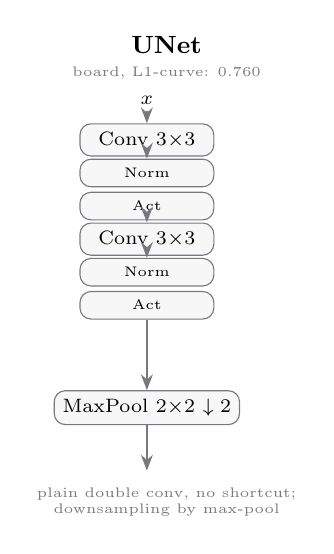
\begin{tikzpicture}[font=\scriptsize]
        \node[font=\small\bfseries] at (0.55,3.65) {UNet};
        \node[font=\tiny,text=soft] at (0.55,3.30) {board, L1-curve: 0.760};
        \node[font=\scriptsize] at (0.3,2.95) {$x$};
        \node[gate,minimum width=17mm] (c1) at (0.3,2.45) {Conv $3{\times}3$};
        \node[gate,minimum width=17mm,minimum height=3.5mm,font=\tiny] (n1) at (0.3,2.03) {Norm};
        \node[gate,minimum width=17mm,minimum height=3.5mm,font=\tiny] (a1) at (0.3,1.61) {Act};
        \node[gate,minimum width=17mm] (c2) at (0.3,1.19) {Conv $3{\times}3$};
        \node[gate,minimum width=17mm,minimum height=3.5mm,font=\tiny] (n2) at (0.3,0.77) {Norm};
        \node[gate,minimum width=17mm,minimum height=3.5mm,font=\tiny] (a2) at (0.3,0.35) {Act};
        \node[gate,minimum width=17mm] (pool) at (0.3,-0.95) {MaxPool $2{\times}2$ $\downarrow 2$};
        \draw[flow,soft] (0.3,2.82) -- (c1.north);
        \draw[flow,soft] (c1.south) -- (n1.north);
        \draw[flow,soft] (a1.south) -- (c2.north);
        \draw[flow,soft] (c2.south) -- (n2.north);
        \draw[flow,soft] (a2.south) -- (pool.north);
        \draw[flow,soft] (pool.south) -- (0.3,-1.75);
        \node[font=\tiny,text=soft,align=center] at (0.55,-2.15) {plain double conv, no shortcut;\\downsampling by max-pool};
      \end{tikzpicture}
    \end{column}
    \begin{column}{0.32\textwidth}
      \centering
      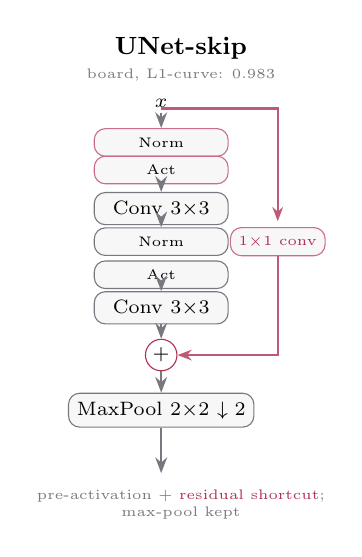
\begin{tikzpicture}[font=\scriptsize]
        \node[font=\small\bfseries] at (0.55,3.65) {UNet-skip};
        \node[font=\tiny,text=soft] at (0.55,3.30) {board, L1-curve: 0.983};
        \node[font=\scriptsize] at (0.3,2.95) {$x$};
        \node[gate,draw=accent!70,minimum width=17mm,minimum height=3.5mm,font=\tiny] (n0) at (0.3,2.45) {Norm};
        \node[gate,draw=accent!70,minimum width=17mm,minimum height=3.5mm,font=\tiny] (a0) at (0.3,2.10) {Act};
        \node[gate,minimum width=17mm] (c1) at (0.3,1.61) {Conv $3{\times}3$};
        \node[gate,minimum width=17mm,minimum height=3.5mm,font=\tiny] (n1) at (0.3,1.19) {Norm};
        \node[gate,minimum width=17mm,minimum height=3.5mm,font=\tiny] (a1) at (0.3,0.77) {Act};
        \node[gate,minimum width=17mm] (c2) at (0.3,0.35) {Conv $3{\times}3$};
        \node[circle,draw=accent,inner sep=1.2pt,font=\scriptsize] (add) at (0.3,-0.25) {$+$};
        \node[gate,minimum width=17mm] (pool) at (0.3,-0.95) {MaxPool $2{\times}2$ $\downarrow 2$};
        \draw[flow,soft] (0.3,2.82) -- (n0.north);
        \draw[flow,soft] (a0.south) -- (c1.north);
        \draw[flow,soft] (c1.south) -- (n1.north);
        \draw[flow,soft] (a1.south) -- (c2.north);
        \draw[flow,soft] (c2.south) -- (add.north);
        \draw[flow,soft] (add.south) -- (pool.north);
        \draw[flow,soft] (pool.south) -- (0.3,-1.75);
        \node[gate,draw=accent!70,text=accent,font=\tiny,minimum height=3.5mm] (sc) at (1.78,1.19) {$1{\times}1$ conv};
        \draw[accent!80,thick,-{Stealth[length=1.8mm]}] (0.3,2.88) -| (1.78,1.45);
        \draw[accent!80,thick,-{Stealth[length=1.8mm]}] (sc.south) |- (add.east);
        \node[font=\tiny,text=soft,align=center] at (0.55,-2.15) {pre-activation + \textcolor{accent}{residual shortcut};\\max-pool kept};
      \end{tikzpicture}
    \end{column}
    \begin{column}{0.32\textwidth}
      \centering
      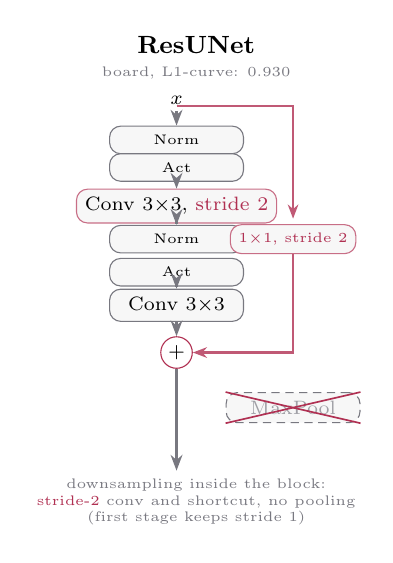
\begin{tikzpicture}[font=\scriptsize]
        \node[font=\small\bfseries] at (0.55,3.65) {ResUNet};
        \node[font=\tiny,text=soft] at (0.55,3.30) {board, L1-curve: 0.930};
        \node[font=\scriptsize] at (0.3,2.95) {$x$};
        \node[gate,minimum width=17mm,minimum height=3.5mm,font=\tiny] (n0) at (0.3,2.45) {Norm};
        \node[gate,minimum width=17mm,minimum height=3.5mm,font=\tiny] (a0) at (0.3,2.10) {Act};
        \node[gate,draw=accent!70,minimum width=17mm] (c1) at (0.3,1.61) {Conv $3{\times}3$, \textcolor{accent}{stride 2}};
        \node[gate,minimum width=17mm,minimum height=3.5mm,font=\tiny] (n1) at (0.3,1.19) {Norm};
        \node[gate,minimum width=17mm,minimum height=3.5mm,font=\tiny] (a1) at (0.3,0.77) {Act};
        \node[gate,minimum width=17mm] (c2) at (0.3,0.35) {Conv $3{\times}3$};
        \node[circle,draw=accent,inner sep=1.2pt,font=\scriptsize] (add) at (0.3,-0.25) {$+$};
        \node[gate,densely dashed,text=soft!70,minimum width=17mm] (ghost) at (1.78,-0.95) {MaxPool};
        \draw[accent,semithick] (ghost.north west) -- (ghost.south east);
        \draw[accent,semithick] (ghost.south west) -- (ghost.north east);
        \draw[flow,soft] (0.3,2.82) -- (n0.north);
        \draw[flow,soft] (a0.south) -- (c1.north);
        \draw[flow,soft] (c1.south) -- (n1.north);
        \draw[flow,soft] (a1.south) -- (c2.north);
        \draw[flow,soft] (c2.south) -- (add.north);
        \draw[flow,soft] (add.south) -- (0.3,-1.75);
        \node[gate,draw=accent!70,text=accent,font=\tiny,minimum height=3.5mm] (sc) at (1.78,1.19) {$1{\times}1$, \textcolor{accent}{stride 2}};
        \draw[accent!80,thick,-{Stealth[length=1.8mm]}] (0.3,2.88) -| (1.78,1.45);
        \draw[accent!80,thick,-{Stealth[length=1.8mm]}] (sc.south) |- (add.east);
        \node[font=\tiny,text=soft,align=center] at (0.55,-2.15) {downsampling inside the block:\\\textcolor{accent}{stride-2} conv and shortcut, no pooling\\(first stage keeps stride 1)};
      \end{tikzpicture}
    \end{column}
  \end{columns}
\end{frame}

% full deck p.102 --- sections/12b_dual.tex
\begin{frame}{The dual model --- two trunks, one head}
  \begin{columns}[c]
    \begin{column}{0.54\textwidth}
      \centering
      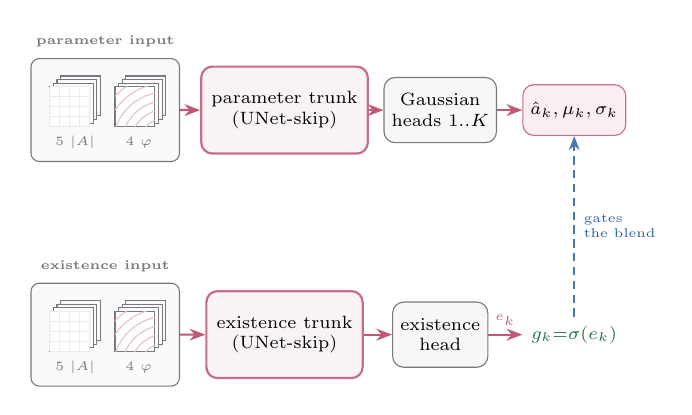
\begin{tikzpicture}[font=\scriptsize, scale=0.92, transform shape,
          exc/.style={-{Stealth[length=1.8mm]}, argA!85, thick, densely dashed}]
        % parameter input card
        \begin{scope}[shift={(0,2.1)}]
          \draw[soft,thin,rounded corners=3pt,fill=black!2] (0,0) rectangle (2.05,1.42);
          \foreach \i in {3,2,1} \draw[soft,thin,fill=black!2] (0.26+0.05*\i,0.48+0.05*\i) rectangle ++(0.55,0.55);
          \draw[soft,thin,fill=white] (0.26,0.48) rectangle ++(0.55,0.55);
          \draw[black!8,xstep=0.1375,ystep=0.1375,shift={(0.26,0.48)}] (0,0) grid (0.55,0.55);
          \foreach \i in {3,2,1} \draw[soft,thin,fill=black!2] (1.16+0.05*\i,0.48+0.05*\i) rectangle ++(0.55,0.55);
          \draw[soft,thin,fill=white] (1.16,0.48) rectangle ++(0.55,0.55);
          \begin{scope} \clip (1.16,0.48) rectangle ++(0.55,0.55); \foreach \r in {0.25,0.37,...,1.2} \draw[accent!30,thin] (1.86,0.23) circle (\r); \end{scope}
          \node[font=\tiny,text=soft] at (0.61,0.26) {5 $|A|$};
          \node[font=\tiny,text=soft] at (1.49,0.26) {4 $\varphi$};
          \node[font=\tiny\bfseries,text=soft,anchor=south] at (1.025,1.45) {parameter input};
        \end{scope}
        % existence input card
        \begin{scope}[shift={(0,-1.0)}]
          \draw[soft,thin,rounded corners=3pt,fill=black!2] (0,0) rectangle (2.05,1.42);
          \foreach \i in {3,2,1} \draw[soft,thin,fill=black!2] (0.26+0.05*\i,0.48+0.05*\i) rectangle ++(0.55,0.55);
          \draw[soft,thin,fill=white] (0.26,0.48) rectangle ++(0.55,0.55);
          \draw[black!8,xstep=0.1375,ystep=0.1375,shift={(0.26,0.48)}] (0,0) grid (0.55,0.55);
          \foreach \i in {3,2,1} \draw[soft,thin,fill=black!2] (1.16+0.05*\i,0.48+0.05*\i) rectangle ++(0.55,0.55);
          \draw[soft,thin,fill=white] (1.16,0.48) rectangle ++(0.55,0.55);
          \begin{scope} \clip (1.16,0.48) rectangle ++(0.55,0.55); \foreach \r in {0.25,0.37,...,1.2} \draw[accent!30,thin] (1.86,0.23) circle (\r); \end{scope}
          \node[font=\tiny,text=soft] at (0.61,0.26) {5 $|A|$};
          \node[font=\tiny,text=soft] at (1.49,0.26) {4 $\varphi$};
          \node[font=\tiny\bfseries,text=soft,anchor=south] at (1.025,1.45) {existence input};
        \end{scope}
        % trunks, heads, outputs
        \node[box, minimum width=21mm, minimum height=12mm] (tp) at (3.5,2.81)  {parameter trunk\\(UNet-skip)};
        \node[box, minimum width=21mm, minimum height=12mm] (te) at (3.5,-0.29) {existence trunk\\(UNet-skip)};
        \node[gate, minimum height=9mm]  (gh) at (5.65,2.81)  {Gaussian\\heads $1..K$};
        \node[gate, minimum height=9mm]  (eh) at (5.65,-0.29) {existence\\head};
        \node[gate, draw=accent!70, fill=accent!8, minimum height=7mm] (op) at (7.5,2.81) {$\hat a_k,\mu_k,\sigma_k$};
        \node[font=\scriptsize, text=good] (gk) at (7.5,-0.29) {$g_k{=}\sigma(e_k)$};
        \draw[flow] (2.05,2.81) -- (tp.west);
        \draw[flow] (2.05,-0.29) -- (te.west);
        \draw[flow] (tp.east) -- (gh.west);
        \draw[flow] (te.east) -- (eh.west);
        \draw[flow] (gh.east) -- (op.west);
        \draw[flow] (eh.east) -- node[midway, above, font=\tiny]{$e_k$} (gk.west);
        \draw[exc] (gk.north) -- node[midway, right, font=\tiny, text=argA, align=left]{gates\\the blend} (op.south);
      \end{tikzpicture}
      \\[8pt]
      {\footnotesize each gate:\; $a_k = g_k\,\hat a_k + (1-g_k)\,a_{\mathrm{off},k}$}\\[1pt]
      {\scriptsize\color{soft} the set-prediction head of Act III, unchanged --- only the source of each embedding splits\par}
    \end{column}
    \begin{column}{0.43\textwidth}
      \small
      \begin{itemize}\setlength{\itemsep}{5pt}
        \item \textbf{Split the encoder, keep the head}: two independent UNet-skip
              trunks --- the Gaussian heads read one embedding, the existence
              head the other. Gate blend and Hungarian matching stay as they are.
        \item \textbf{Each trunk picks its own stack}: the channel groups $|A|$
              (5 amplitudes) and $\varphi$ (4 interferograms) are selected
              per trunk --- which modality reaches which head becomes an
              architectural choice.
        \item \textbf{Why route}: the input ablation split the labour --- phase
              fires the slots, the full stack calibrates the parameters. The
              dual model can hand each head the input its job needs.
      \end{itemize}
    \end{column}
  \end{columns}
\end{frame}

% full deck p.123 --- sections/12b_dual.tex
\begin{frame}{Pairing the objective --- param-L1 plus a curve term}
  \begin{columns}[c]
    \begin{column}{0.53\textwidth}
      \centering
      $\mathcal{L}(w) \;=\; \bigl(\mathcal{L}_{\text{param-L1}} \,+\, w\,\mathcal{L}_{\text{curve}}\bigr)\,/\,(1+w)$
      \\[10pt]
      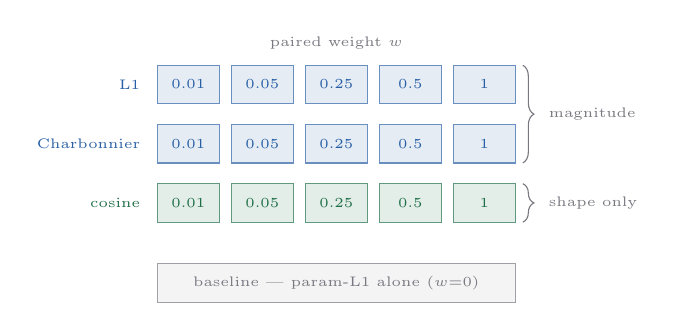
\begin{tikzpicture}[font=\scriptsize, scale=0.94]
        \node[font=\tiny,text=soft] at (3.5,2.42) {paired weight $w$};
        \foreach \y/\fam/\col in {1.6/L1/argA, 0.8/Charbonnier/argA, 0.0/cosine/good}{
          \node[font=\tiny,text=\col,anchor=east] at (0.98,\y+0.26) {\fam};
        }
        \foreach \x/\w in {1.5/0.01, 2.5/0.05, 3.5/0.25, 4.5/0.5, 5.5/1}{
          \foreach \y/\col in {1.6/argA, 0.8/argA, 0.0/good}{
            \draw[\col!70,thin,fill=\col!12] (\x-0.42,\y) rectangle (\x+0.42,\y+0.52);
            \node[font=\tiny,text=\col] at (\x,\y+0.26) {\w};
          }
        }
        \draw[decorate,decoration={brace,amplitude=4pt},soft] (6.02,2.12) -- (6.02,0.8);
        \node[font=\tiny,text=soft,anchor=west] at (6.24,1.46) {magnitude};
        \draw[decorate,decoration={brace,amplitude=4pt},soft] (6.02,0.52) -- (6.02,0.0);
        \node[font=\tiny,text=soft,anchor=west] at (6.24,0.26) {shape only};
        \draw[soft!70,thin,fill=soft!8] (1.08,-1.08) rectangle (5.92,-0.56);
        \node[font=\tiny,text=soft] at (3.5,-0.82) {baseline --- param-L1 alone ($w{=}0$)};
      \end{tikzpicture}
      \\[7pt]
      {\scriptsize\color{soft} 1 baseline $+$ 15 pair arms per $K$, five seeds each, at $K{=}2$ and $K{=}5$ $=$ 160 runs\par}
    \end{column}
    \begin{column}{0.43\textwidth}
      \footnotesize
      The ratio block left the $K{=}5$ gate under-firing at every split ---
      more existence capacity did not wake it. This experiment changes the
      objective instead: keep param-L1 and add a synthesized-curve term.
      \par\smallskip
      \begin{itemize}\setlength{\itemsep}{3pt}
        \item \textbf{Two signals, one loss}: param-L1 reaches a slot only
              through its matched pair; the curve term re-synthesizes the
              profile from \emph{all} slots and is permutation-invariant ---
              its gradient touches every slot, matched or not.
        \item \textbf{Magnitude or shape}: L1 and Charbonnier price the
              synthesized profile's magnitude; cosine normalizes both curves
              first and prices shape alone.
        \item \textbf{A normalized pair}: the two terms are averaged, so the
              validation loss changes meaning with $w$ --- arms compare on
              held-out metrics only, never on the loss.
        \item \textbf{The question}: if the conservative gate is starved of a
              profile-level error signal rather than capacity, a small $w$
              should move detection at $K{=}5$ and leave $K{=}2$ alone.
      \end{itemize}
    \end{column}
  \end{columns}
\end{frame}

% next-steps agenda (short deck only)
\begin{frame}{Next steps}
  \begin{itemize}\setlength{\itemsep}{16pt}
    \item \textbf{Physical loss terms}: the five ranked terms on the next three frames: covariance matching, coherence re-synthesis, moments, total power, the Capon cycle.
    \item \textbf{$\gamma$-net adaptation}: adapting the $\gamma$-net architecture to this pipeline.
    \item \textbf{JEPA pretraining}: predicting in representation space, the closing frame.
  \end{itemize}
\end{frame}

% full deck p.134 --- sections/13_physics_losses.tex
\begin{frame}{Data-consistency terms (the ranked top two)}
  \setlength{\abovedisplayskip}{3pt}
  \setlength{\belowdisplayskip}{3pt}
  \begin{columns}[T]
    \begin{column}{0.46\textwidth}
      \begin{minipage}[t][0.78\textheight][s]{\linewidth}
      \centering
      \textbf{Coherence re-synthesis}\\[1pt]
      {\footnotesize\color{soft} coherence domain}
      \par\vfill
      \[
        \gamma_P(k_z^{(i)}) = \frac{\sum_n P(\xi_n)\, e^{j k_z^{(i)} \xi_n}}{\sum_n P(\xi_n)}
      \]
      \[
        \ell_{\text{coh}} = \Big\langle \tfrac{1}{N_s}\textstyle\sum_i
          \big| \gamma_P(k_z^{(i)}) - \gamma_T(k_z^{(i)}) \big|^2 \Big\rangle
      \]
      \par\vfill
      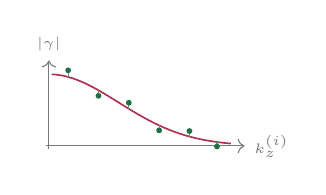
\begin{tikzpicture}[scale=0.70]
        \draw[->,soft] (-0.05,0) -- (3.55,0) node[right,font=\tiny]{$k_z^{(i)}$};
        \draw[->,soft] (0,-0.05) -- (0,1.55) node[above,font=\tiny]{$|\gamma|$};
        \draw[accent,semithick,domain=0.05:3.3,samples=60,smooth] plot (\x,{1.3*exp(-\x*\x/3.2)});
        \foreach \x/\d in {0.35/0.12, 0.9/-0.10, 1.45/0.11, 2.0/-0.09, 2.55/0.10, 3.05/-0.08} {
          \draw[good!70,thin] (\x,{1.3*exp(-\x*\x/3.2)}) -- (\x,{1.3*exp(-\x*\x/3.2)+\d});
          \fill[good] (\x,{1.3*exp(-\x*\x/3.2)+\d}) circle (1.5pt);
        }
      \end{tikzpicture}
      \\[4pt]
      {\scriptsize \textcolor{accent}{$\gamma_P$ from the predicted mixture} pulled onto
       \textcolor{good}{the target coherences}, baseline by baseline.}
      \par\vfill
      {\footnotesize Cloude 2006 (PCT); same Fourier kernel as gamma-Net (Qian et al.).}
      \end{minipage}
    \end{column}
    \begin{column}{0.02\textwidth}
      \centering
      \textcolor{soft!40}{\rule{0.4pt}{0.74\textheight}}
    \end{column}
    \begin{column}{0.46\textwidth}
      \begin{minipage}[t][0.78\textheight][s]{\linewidth}
      \centering
      \textbf{Covariance matching}\\[1pt]
      {\footnotesize\color{soft} covariance domain}
      \par\vfill
      \[
        \mathbf{R}[P] = \mathbf{A}\,\mathrm{diag}(P)\,\mathbf{A}^{H} \Delta\xi
      \]
      \[
        \ell_{\text{cov}} = \Big\langle
          \tfrac{\| \mathbf{R}[P] - \mathbf{R}[T] \|_F^2}{\| \mathbf{R}[T] \|_F^2} \Big\rangle
      \]
      \par\vfill
      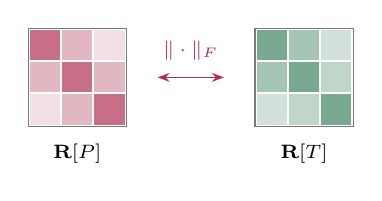
\begin{tikzpicture}[scale=1.2]
        \foreach \i/\j/\c in {0/2/70,1/2/35,2/2/15,0/1/35,1/1/70,2/1/35,0/0/15,1/0/35,2/0/70}
          \fill[accent!\c] (\i*0.34,\j*0.34) rectangle ++(0.32,0.32);
        \draw[soft,thin] (-0.02,-0.02) rectangle (1.02,1.02);
        \node[font=\scriptsize,anchor=north] at (0.5,-0.1) {$\mathbf{R}[P]$};
        \draw[{Stealth[length=1.5mm]}-{Stealth[length=1.5mm]},accent,semithick] (1.35,0.5) -- (2.05,0.5);
        \node[font=\scriptsize,text=accent,anchor=south] at (1.7,0.58) {$\|\cdot\|_F$};
        \begin{scope}[shift={(2.4,0)}]
          \foreach \i/\j/\c in {0/2/60,1/2/40,2/2/20,0/1/40,1/1/60,2/1/28,0/0/20,1/0/28,2/0/60}
            \fill[good!\c] (\i*0.34,\j*0.34) rectangle ++(0.32,0.32);
          \draw[soft,thin] (-0.02,-0.02) rectangle (1.02,1.02);
          \node[font=\scriptsize,anchor=north] at (0.5,-0.1) {$\mathbf{R}[T]$};
        \end{scope}
      \end{tikzpicture}
      \\[4pt]
      {\scriptsize \textcolor{accent}{Synthesised} vs \textcolor{good}{target} covariance ---
       structure and relative scale, entry by entry.}
      \par\vfill
      {\footnotesize COMET (Ottersten, Stoica, Roy 1998); TomoSAR: Cros \& Ferro-Famil 2025;
       CS fidelity: Berenger et al. 2023.}
      \end{minipage}
    \end{column}
  \end{columns}
\end{frame}

% full deck p.135 --- sections/13_physics_losses.tex
\begin{frame}{Descriptor terms: moments and total power}
  \setlength{\abovedisplayskip}{3pt}
  \setlength{\belowdisplayskip}{3pt}
  \begin{columns}[T]
    \begin{column}{0.46\textwidth}
      \centering
      \textbf{Moments}\\[1pt]
      {\footnotesize\color{soft} mass \; $\cdot$ \; phase-centre $\bar z$ \; $\cdot$ \; spread $\sigma_z$}
      \\[6pt]
      \[
        m = \textstyle\sum_n P(\xi_n)\,\Delta\xi
      \]
      \[
        \bar z = \tfrac{\sum_n \xi_n P(\xi_n)}{\sum_n P(\xi_n)}, \qquad
        \sigma_z^2 = \tfrac{\sum_n (\xi_n-\bar z)^2 P(\xi_n)}{\sum_n P(\xi_n)}
      \]
      \vspace{15pt}
      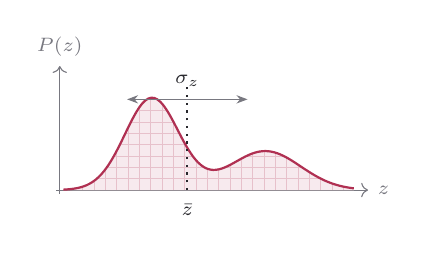
\begin{tikzpicture}[scale=0.9]
        \draw[->,soft] (-0.05,0) -- (4.35,0) node[right,font=\scriptsize]{$z$};
        \draw[->,soft] (0,-0.05) -- (0,1.75) node[above,font=\scriptsize]{$P(z)$};
        \fill[accent!10] plot[domain=0.05:4.15,samples=80,smooth]
          (\x,{1.3*exp(-(\x-1.3)^2/(2*0.38*0.38))+0.55*exp(-(\x-2.9)^2/(2*0.5*0.5))})
          -- (4.15,0) -- (0.05,0) -- cycle;
        \begin{scope}
          \clip plot[domain=0.05:4.15,samples=80,smooth]
            (\x,{1.3*exp(-(\x-1.3)^2/(2*0.38*0.38))+0.55*exp(-(\x-2.9)^2/(2*0.5*0.5))})
            -- (4.15,0) -- (0.05,0) -- cycle;
          \draw[accent!30,very thin,step=0.16] (0,0) grid (4.2,1.6);
        \end{scope}
        \draw[accent,thick,domain=0.05:4.15,samples=100,smooth]
          plot (\x,{1.3*exp(-(\x-1.3)^2/(2*0.38*0.38))+0.55*exp(-(\x-2.9)^2/(2*0.5*0.5))});
        \draw[ink,dotted,thick] (1.8,0) -- (1.8,1.5);
        \node[font=\scriptsize,text=ink,anchor=north] at (1.8,-0.06) {$\bar z$};
        \draw[{Stealth[length=1.4mm]}-{Stealth[length=1.4mm]},soft,thin] (0.95,1.28) -- (2.65,1.28);
        \node[font=\scriptsize,text=ink,anchor=south] at (1.8,1.33) {$\sigma_z$};
      \end{tikzpicture}
      \\[2pt]
      {\scriptsize Centroid and spread are bias-robust \emph{ratios}
       (Cros \& Ferro-Famil 2025).}
    \end{column}
    \begin{column}{0.02\textwidth}
      \centering
      \textcolor{soft!40}{\rule{0.4pt}{0.58\textheight}}
    \end{column}
    \begin{column}{0.46\textwidth}
      \centering
      \textbf{Total power}\\[1pt]
      {\footnotesize\color{soft} the one absolute-power quantity}
      \\[6pt]
      \[
        P_{\text{tot}}[\,\cdot\,] = \textstyle\sum_n (\,\cdot\,)(\xi_n)\,\Delta\xi
      \]
      \[
        \ell_{\text{pow}} = \Big\langle \big( P_{\text{tot}}[P] - P_{\text{tot}}[T] \big)^2 \Big\rangle
      \]
      \vspace{15pt}
      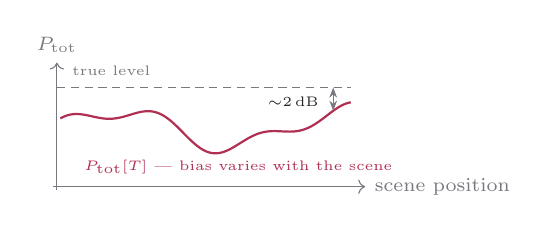
\begin{tikzpicture}[scale=0.9]
        \draw[->,soft] (-0.05,0) -- (4.35,0) node[right,font=\scriptsize]{scene position};
        \draw[->,soft] (0,-0.05) -- (0,1.75) node[above,font=\scriptsize]{$P_{\text{tot}}$};
        \draw[soft,densely dashed] (0,1.4) -- (4.15,1.4);
        \node[font=\tiny,text=soft,anchor=south west] at (0.08,1.43) {true level};
        \draw[accent,thick,domain=0.05:4.15,samples=120,smooth]
          plot (\x,{0.82+0.26*sin(\x*110)+0.12*sin(\x*260+70)});
        \node[font=\tiny,text=accent,anchor=west] at (0.25,0.28)
          {$P_{\text{tot}}[T]$ --- bias varies with the scene};
        \draw[{Stealth[length=1.3mm]}-{Stealth[length=1.3mm]},soft,thin] (3.9,1.07) -- (3.9,1.4);
        \node[font=\tiny,text=ink,anchor=east] at (3.83,1.2) {$\sim$2\,dB};
      \end{tikzpicture}
      \\[2pt]
      {\scriptsize The target $P_{\text{tot}}[T]$ is not the true power: its bias moves with
       scene content (Lopez-Dekker \& Mallorqui 2010) --- the loss would imprint that bias.}
    \end{column}
  \end{columns}
\end{frame}

% full deck p.136 --- sections/13_physics_losses.tex
\begin{frame}{The estimator-cycle term: Capon cycle}
  \setlength{\abovedisplayskip}{4pt}
  \setlength{\belowdisplayskip}{4pt}
  \small
  Push the prediction through the \emph{same estimator} that produced the ground truth:
  \[
    \hat T_P(\xi_n) = \big( \mathbf{a}^{H}(\xi_n)
      (\mathbf{R}[P] + \epsilon\bar\sigma\mathbf{I})^{-1} \mathbf{a}(\xi_n) \big)^{-1}
  \]
  \vspace{8pt}
  \begin{center}
  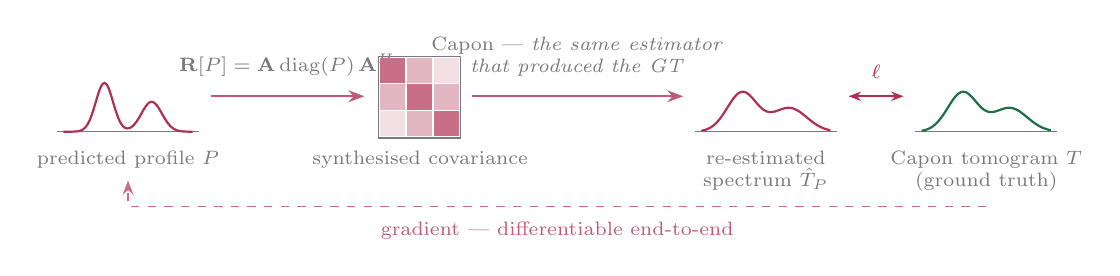
\begin{tikzpicture}
    \draw[soft,thin] (0,0) -- (1.8,0);
    \draw[accent,thick,domain=0.08:1.72,samples=70,smooth]
      plot (\x,{0.62*exp(-(\x-0.6)^2/(2*0.11*0.11))+0.38*exp(-(\x-1.2)^2/(2*0.13*0.13))});
    \node[font=\scriptsize,text=soft,anchor=north] at (0.9,-0.12) {predicted profile $P$};
    \draw[flow] (1.95,0.45) -- (3.9,0.45);
    \node[font=\scriptsize,text=soft,anchor=south] at (2.92,0.58)
      {$\mathbf{R}[P]=\mathbf{A}\,\mathrm{diag}(P)\,\mathbf{A}^{H}$};
    \begin{scope}[shift={(4.1,-0.06)}]
      \foreach \i/\j/\c in {0/2/70, 1/2/35, 2/2/15, 0/1/35, 1/1/70, 2/1/35, 0/0/15, 1/0/35, 2/0/70}
        \fill[accent!\c] (\i*0.34,\j*0.34) rectangle ++(0.32,0.32);
      \draw[soft,thin] (-0.02,-0.02) rectangle (1.02,1.02);
    \end{scope}
    \node[font=\scriptsize,text=soft,anchor=north] at (4.61,-0.12) {synthesised covariance};
    \draw[flow] (5.27,0.45) -- (7.95,0.45);
    \node[font=\scriptsize,text=soft,anchor=south,align=center] at (6.61,0.58)
      {Capon --- \emph{the same estimator}\\\emph{that produced the GT}};
    \draw[soft,thin] (8.1,0) -- (9.9,0);
    \draw[accent,thick,domain=8.18:9.82,samples=70,smooth]
      plot (\x,{0.50*exp(-(\x-8.7)^2/(2*0.19*0.19))+0.30*exp(-(\x-9.3)^2/(2*0.22*0.22))});
    \node[font=\scriptsize,text=soft,anchor=north,align=center] at (9.0,-0.12)
      {re-estimated\\spectrum $\hat T_P$};
    \draw[{Stealth[length=1.6mm]}-{Stealth[length=1.6mm]},accent,semithick] (10.05,0.45) -- (10.75,0.45);
    \node[font=\scriptsize,text=accent,anchor=south] at (10.4,0.55) {$\ell$};
    \draw[soft,thin] (10.9,0) -- (12.7,0);
    \draw[good,thick,domain=10.98:12.62,samples=70,smooth]
      plot (\x,{0.50*exp(-(\x-11.5)^2/(2*0.19*0.19))+0.30*exp(-(\x-12.1)^2/(2*0.22*0.22))});
    \node[font=\scriptsize,text=soft,anchor=north,align=center] at (11.8,-0.12)
      {Capon tomogram $T$\\(ground truth)};
    \draw[accent!70,dashed,-{Stealth[length=1.8mm]}] (11.8,-0.95) -- (0.9,-0.95) -- (0.9,-0.62);
    \node[font=\scriptsize,text=accent!80,anchor=north] at (6.35,-1.02)
      {gradient --- differentiable end-to-end};
  \end{tikzpicture}
  \end{center}
  \vspace{6pt}
  \begin{itemize}
    \item Absorbs the Capon bias and the PSF \textbf{by construction}.
    \item Costs an $N_s\times N_s$ solve per pixel --- the most expensive of the five.
  \end{itemize}
  \vspace{2pt}
  {\scriptsize\color{soft} Cycle-consistency lineage: Yaman 2020, Lu 2021,
   Vella \& Mota 2020, Angermann 2023.\par}
\end{frame}

% full deck p.140 --- sections/14_unrolled.tex
\begin{frame}{The unrolled model: the solver becomes the network}
  \centering
  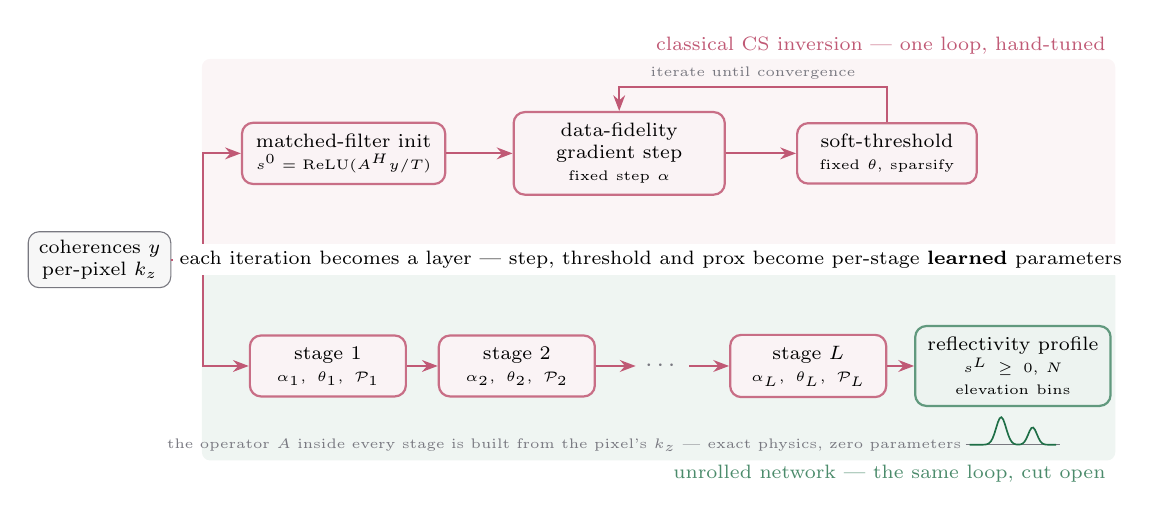
\begin{tikzpicture}
    \begin{scope}[on background layer]
      \fill[accent!5,rounded corners=3pt] (1.3,0.10)  rectangle (12.9,2.55);
      \fill[good!7,rounded corners=3pt]   (1.3,-0.10) rectangle (12.9,-2.55);
      \draw[soft!50,dotted] (-0.9,0) -- (12.9,0);
    \end{scope}
    \node[font=\scriptsize,text=accent!80,anchor=east] at (12.9,2.72)  {classical CS inversion --- one loop, hand-tuned};
    \node[font=\scriptsize,text=good!80,anchor=east]   at (12.9,-2.72) {unrolled network --- the same loop, cut open};
    \node[gate, text width=16mm] (in) at (0,0) {coherences $y$\\per-pixel $k_z$};
    \node[box, text width=23mm] (init) at (3.1,1.35)  {matched-filter init\\{\tiny $s^{0}=\mathrm{ReLU}(A^{H}y/T)$}};
    \node[box, text width=24mm] (grad) at (6.6,1.35)  {data-fidelity gradient step\\{\tiny fixed step $\alpha$}};
    \node[box, text width=20mm] (thr)  at (10.0,1.35) {soft-threshold\\{\tiny fixed $\theta$, sparsify}};
    \draw[flow] (in.east) -- ++(0.4,0) |- (init.west);
    \draw[flow] (init) -- (grad);
    \draw[flow] (grad) -- (thr);
    \draw[flow] (thr.north) -- ++(0,0.45) -| (grad.north);
    \node[font=\tiny, text=soft, anchor=south] at (8.3,2.17) {iterate until convergence};
    \node[box, text width=17mm] (st1) at (2.9,-1.35) {stage 1\\{\tiny $\alpha_1,\ \theta_1,\ \mathcal{P}_1$}};
    \node[box, text width=17mm] (st2) at (5.3,-1.35) {stage 2\\{\tiny $\alpha_2,\ \theta_2,\ \mathcal{P}_2$}};
    \node[font=\small, text=soft] (dots) at (7.15,-1.35) {$\cdots$};
    \node[box, text width=17mm] (stL) at (9.0,-1.35) {stage $L$\\{\tiny $\alpha_L,\ \theta_L,\ \mathcal{P}_L$}};
    \node[box, draw=good!70, fill=good!8, text width=22mm] (out) at (11.6,-1.35) {reflectivity profile\\{\tiny $s^{L}\ge 0$, $N$ elevation bins}};
    \draw[soft,thin] (11.0,-2.35) -- (12.2,-2.35);
    \draw[good,semithick] plot[domain=11.05:12.15,samples=50] (\x,{-2.35+0.35*exp(-(\x-11.45)^2/0.008)+0.22*exp(-(\x-11.85)^2/0.006)});
    \draw[flow] (in.east) -- ++(0.4,0) |- (st1.west);
    \draw[flow] (st1) -- (st2);
    \draw[flow] (st2) -- (dots);
    \draw[flow] (dots) -- (stL);
    \draw[flow] (stL) -- (out);
    \node[font=\tiny, text=soft, anchor=north] at (5.9,-2.15)
      {the operator $A$ inside every stage is built from the pixel's $k_z$ --- exact physics, zero parameters};
    \node[font=\scriptsize, fill=white, inner sep=2.5pt] at (7.0,0)
      {each iteration becomes a layer --- step, threshold and prox become per-stage \textbf{learned} parameters};
  \end{tikzpicture}
  \\[2pt]
  \vspace{-4pt}
  \[
    r^{\ell} \;=\; s^{\ell} + \alpha_\ell\,\mathrm{Re}\!\big[A^{H}(y - A s^{\ell})\big]/L_{\mathrm{lip}},
    \qquad
    s^{\ell+1} \;=\; \mathrm{ReLU}\!\big(\mathcal{P}_\ell(r^{\ell}) - \theta_\ell\big)
  \]
  {\scriptsize $\gamma$-Net lineage (Qian et al., IEEE TGRS 2022); LISTA (Gregor \& LeCun 2010); ISTA-Net (Zhang \& Ghanem 2018).
   $\mathcal{P}_\ell$: per-pixel residual 1D convolution along elevation; $L_{\mathrm{lip}} = TN\,\mathrm{d}z^{2}$ normalises the step.
   Default $L{=}8$: $\sim$1.4k parameters.}
\end{frame}

% full deck p.145 --- sections/15_jepa.tex
\begin{frame}{What JEPA does}
  \centering
  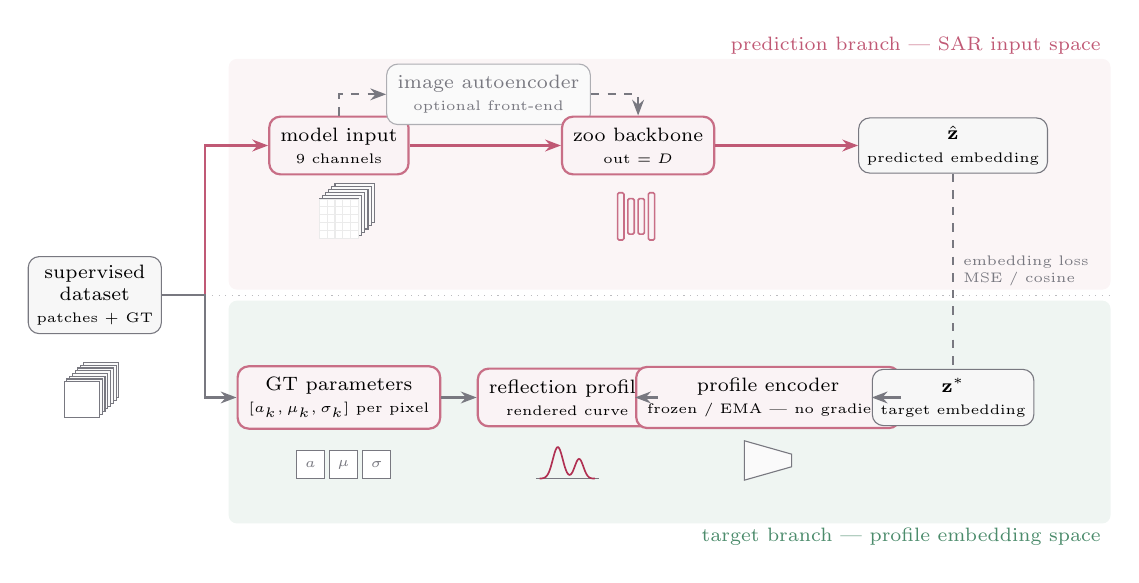
\begin{tikzpicture}
    \begin{scope}[on background layer]
      \fill[accent!5,rounded corners=3pt] (1.7,0.07) rectangle (12.9,3.0);
      \fill[good!7,rounded corners=3pt] (1.7,-0.07) rectangle (12.9,-2.9);
      \draw[soft!50,dotted] (-0.2,0) -- (12.9,0);
    \end{scope}
    \node[font=\scriptsize,text=accent!80,anchor=east] at (12.9,3.17) {prediction branch --- SAR input space};
    \node[font=\scriptsize,text=good!80,anchor=east] at (12.9,-3.07) {target branch --- profile embedding space};
    \node[gate] (ds) at (0,0) {supervised\\dataset\\{\tiny patches + GT}};
    \foreach \i in {7,6,5,4,3,2,1} \draw[soft,thin,fill=black!2] (-0.39+0.035*\i,-1.55+0.035*\i) rectangle ++(0.45,0.45);
    \draw[soft,thin,fill=white] (-0.39,-1.55) rectangle ++(0.45,0.45);
    \node[box] (top1) at (3.1,1.9) {model input\\{\tiny 9 channels}};
    \foreach \i in {5,4,3,2,1} \draw[soft,thin,fill=black!2] (2.85+0.04*\i,0.72+0.04*\i) rectangle ++(0.5,0.5);
    \draw[soft,thin,fill=white] (2.85,0.72) rectangle ++(0.5,0.5);
    \draw[black!8,step=0.1,shift={(2.85,0.72)}] (0,0) grid (0.5,0.5);
    \node[ghost] (iae) at (5.0,2.55) {image autoencoder\\{\tiny optional front-end}};
    \node[box] (bb) at (6.9,1.9) {zoo backbone\\{\tiny out $= D$}};
    \foreach \x/\y/\h in {6.64/0.70/0.6,6.77/0.775/0.45,6.90/0.775/0.45,7.03/0.70/0.6} \draw[accent!70,semithick,fill=accent!6,rounded corners=0.5pt] (\x,\y) rectangle ++(0.08,\h);
    \node[gate] (zh) at (10.9,1.9) {$\hat{\mathbf z}$\\{\tiny predicted embedding}};
    \node[box] (bot1) at (3.1,-1.3) {GT parameters\\{\tiny $[a_k,\mu_k,\sigma_k]$ per pixel}};
    \foreach \x/\lbl in {2.56/{$a$},2.98/{$\mu$},3.40/{$\sigma$}} { \draw[soft,thin,fill=white] (\x,-2.33) rectangle ++(0.36,0.36); \node[font=\tiny,text=soft] at (\x+0.18,-2.15) {\lbl}; }
    \node[box] (bot2) at (6.0,-1.3) {reflection profile\\{\tiny rendered curve}};
    \draw[soft,thin] (5.6,-2.33) -- (6.4,-2.33);
    \draw[accent,semithick] plot[domain=5.65:6.35,samples=60] (\x,{-2.33+0.4*exp(-(\x-5.88)^2/0.008)+0.25*exp(-(\x-6.15)^2/0.006)});
    \node[box] (enc) at (8.55,-1.3) {profile encoder\\{\tiny frozen / EMA --- no gradient}};
    \draw[soft,thin,fill=black!2] (8.25,-2.35) -- (8.85,-2.18) -- (8.85,-2.02) -- (8.25,-1.85) -- cycle;
    \node[gate] (zs) at (10.9,-1.3) {$\mathbf z^{*}$\\{\tiny target embedding}};
    \draw[flow] (ds.east) -- ++(0.55,0) |- (top1.west);
    \draw[flow, soft] (ds.east) -- ++(0.55,0) |- (bot1.west);
    \draw[flow] (top1) -- (bb);
    \draw[flow] (bb) -- (zh);
    \draw[flow, soft, dashed] (top1.north) |- (iae);
    \draw[flow, soft, dashed] (iae) -| (bb.north);
    \draw[flow, soft] (bot1) -- (bot2);
    \draw[flow, soft] (bot2) -- (enc);
    \draw[flow, soft] (enc) -- (zs);
    \draw[soft, thick, dashed] (zh) -- node[right, font=\tiny, align=left]{embedding loss\\MSE / cosine} (zs);
  \end{tikzpicture}
  \\[8pt]
  \small
  A network learns to predict, from the reduced stack alone, the \textbf{embedding} that a\\
  separately-trained profile autoencoder assigns to the ground-truth reflection profile.
\end{frame}

\end{document}
